\documentclass[12pt,a4paper,titlepage]{article}
\usepackage[italian]{babel}
\usepackage[T1]{fontenc}
\usepackage[latin1]{inputenc}
\usepackage{titlesec}
\usepackage[hidelinks]{hyperref}
\usepackage[a4paper,top=2cm,bottom=2cm,left=1cm,right=1cm]{geometry}
\usepackage{soulutf8,color}
\usepackage{emptypage}                     
\usepackage{fancyhdr}
\usepackage{graphicx}
\usepackage{float}
\usepackage{array}
\usepackage{longtable}
\usepackage{pgffor}
\pagestyle{fancy}
\newcommand{\minitab}[2][1]{\begin{tabular}#1 #2\end{tabular}}
\newcommand{\uc}[1]{\hyperref[UC#1]{UC#1}}
\begin{document}
	
	\title{ANALISI DEI REQUISITI}
	\author{SWEg Group}
	\date{}
	\maketitle
	
	\lhead{SWEg Group}
	\chead{}
	\lfoot{Analisi dei Requisiti}
	\cfoot{}
	\rfoot{\thepage}
	\renewcommand{\headrulewidth}{0.2pt}
	\renewcommand{\footrulewidth}{0.2pt}
	\rhead{Registro Modifiche}
	\section{Registro Modifiche}
	\small %rippicciolisce il testo
	
	{\renewcommand\arraystretch{1.2}  %aumenta l'altezza di ogni riga
		\begin{tabular}{|l|c|c|c|}
			\hline
			{\textbf{Modifica}}&{\textbf{Nome}}&{\textbf{Data}}&{\textbf{Ver.}}\\
			\hline
			Creazione Raw Documento & Gianluca Crivellaro & 21/12/2016 & 0.0.1 \\
			\hline
			Modifica Raw & Gianluca Crivellaro & 22/12/2016 & 0.0.2 \\
			\hline
			Aggiunti Requisiti & Sebastiano Marchesini & 23/12/2016 & 0.0.3 \\
			\hline
			Aggiunti Requisiti Estesi Concordati & Gianluca Crivellaro & 27/12/2016 & 0.0.4 \\
			\hline
			Stesura Documento (Introduzione) & Sebastiano Marchesini &  28/12/2016 & 0.1.0 \\
			\hline
			Creazione Grafici Use Case & Pietro Lonardi e Gianluca C. & 29/12/2016 & 0.1.1 \\
			\hline
			Stesura Documento (Descrizione Generale \& Casi d'Uso) & Sebastiano Marchesini & 30/12/2016 & 0.1.2 \\
			\hline
			Creazione Grafici Use Case & Pietro Lonardi & 02/01/2017 & 0.1.3 \\
			\hline
			Verifica Documento \& Grafici Use Case & Piergiorgio Danieli & 03/01/2017 & 0.2.0 \\
			\hline
			Tracciamento Requisiti - Fonti e Fonti -Requisiti & Crivellaro Gianluca & 05/01/2017 & 0.3.0\\
			
			\hline
		\end{tabular}
	}	\normalsize
	\newpage
	\rhead{Indice}
	\tableofcontents
	\thispagestyle{empty}
	
	\newpage
	
	
	
	\rhead{Introduzione}
	\section{Introduzione}
	\subsection{Scopo del Documento}
	Tale documento ha lo scopo di studiare e modellare concettualmente il problema che si pone con APIM. Posizionando le componeti (o ambiti) a scopo di allocazione dei requisiti. Alcuni dei requisiti specificandoli con il diagramma dei casi d'uso.
	
	Vi deve essere la certezza di non aver dimenticato nessuno tra i bisogno espliciti ed i bisogni impliciti. Questo implica che non vi sia ambiguità tra i requisiti.
	Bisogna sempre tener conto di portare al massimo possibile la granularità del problema, senza però confonderlo e renderlo impossibile da verificare. Questo per rendere il requisito decidibile.
	
	E' infine bene tener presente otto semplici qualità di selezione dei requisiti:
	\begin{itemize}
		\item Non Ambigui
		\item Corretti
		\item Completi
		\item Verificabili
		\item Consistenti
		\item Modificabili
		\item Tracciabili
		\item Ordinati per Rilevanza
	\end{itemize}
	\subsection{Scopo del Prodotto}
	L'obbiettivo è creare un'infrastruttura che permetta la distribuzione digitale e la gestione dei diritti digitali di microservizi. Creati ed importati da diversi utenti che possono interfacciarsi tra loro.
	
	Viene usata per gestire e distribuire una vasta gamma di microservizi (alcuni esclusivi) ed il loro relativo supporto. Tutte queste operazioni sono effettuate via Internet.
	E' inoltre possibile il monitoraggio di ogni API grazie alle tecnologie fornite dal prodotto. 
	\subsection{Glossario}
	Alla fine di evitare ambiguità e mantenere la consistenza il Glossario è un documento unico e consultabile separatamente.
	
	Un glossario è una raccolta di termini di un ambito specifico e circoscritto. In questo caso per raccogliere termini desueti e specialistici inerenti al progetto. 
	\subsection{Riferimenti}
	\subsubsection{Normativi}
	\begin{itemize}
		\item \textbf{Norme di Progetto}:	"Norme di Progetto v1.0.0".
		\item \textbf{Capitolato d'appalto C1}:	API Market per microservizi \\
		\textcolor{blue}{\url{www.math.unipd.it/~tullio/IS-1/2016/Progetto/C1.pdf}}. 
		\item \textbf{Verbali}:
		\subsubsection{Informativi}
		\item \textbf {Studio di Fattibilità}: "Studio di Fattibilità v.1.0.0".
		\item \textbf{IEEE 830-1998}: Recommended Practice for Software Requirements Specifica- tions \\
		\textcolor{blue}{\url{https://en.wikipedia.org/wiki/Software_requirements_specification}}.
	\end{itemize}
	
	\newpage
	
	\rhead{Descrizione Generale}
	\section{Descrizione Generale}
	\subsection{Obbiettivi del prodotto}
	L'obbiettivo primario del prodotto é di dare ad ogni utente la possibilità di registrare il proprio microservizio in una piattaforma dedicata. In questo modo è possibile la vendita (o condivisione) con gli altri utenti della comunità regolata da politiche di compravendita specifiche e flessibili a seconda dello scopo dell'API o del volere del tecnico. 
	
	L'obbiettivo è quindi quello di incentivare la programmazione a microservizi e, oltre a spingere i gruppi più piccoli nel progettare per il mercato virtuale, pensare sempre di più a delle migliori architetture flessibili invece che veri e propri programmi. Si vogliono abbandonare i vecchi programmi monolite per entrare in una realtà fatta di sistemi divisi in moduli, la nuova sfida progettuale sarà quindi unire i vari microservizi (o API) per costruire un prodotto completo.
	\subsection{Funzioni del prodotto}
	SWEg Group si impegna in particolar modo alle sottoscritte funzioni del prodotto :
	\begin{enumerate}
		\item \textbf{Registrare le API di un microservizio}:	dando la possibilità di caricare un'interfaccia e documentando la propria progettazione.
		\item \textbf{Permetta di consultare le API}:	con un sistema di ricerca designato e filtrato anche con dati tecnici. Pure se con minori funzionalità anche un utente non registrato alla piattaforma può vagliare le varie API. Per ogni API sarà inoltre possibile un consulto dei suoi dati tecnici.
		\item \textbf{Permetta di associare diverse API key}: così da regolare le politiche di scambio dei microservizi. Le API key sono lo strumento principale di collegamento tra la API ed il suo utilizzatore. Grazie a queste l'infrastruttura potrà regolare le scadenze, l'utilizzo ed il procedimento oltre ad avere un ID univoco per la monitorizzazione. 
		\item \textbf{Permetta di monitorare l'utilizzo delle API}:	già accennato nei punti precedenti. Vogliamo che tale infrastruttura tenga conto di particolari dati tecnici di ogni API per renderle così misurabili in termini di efficacia ed efficienza. Oltre che ad avere così un sistema automatizzato per il confronto tra i vari microservizi.
		\item \textbf{Blocchi le chiamate di utenti in possesso di API key scadute e/o non valide}:	è la sottolineatura di uno dei motivi di esistenza delle API key. Punto focale per la regolamentazione dello scambio è la possibilità di acquisto delle chiavi secondo tempo, mole di scambio di dati , eccetera. I dati tecnici per le policy di durata e validità saranno descritte in seguito, ma queste decideranno se è ancora attiva una chiave o meno.
		\item \textbf{Permetta di visualizzare i dati tecnici d'uso delle singole API}:	dopo aver monitorato ogni singola API è possibile fare la stima e produrre un elaborato tecnico dei valori di quest'ultima. E' compito dell'API Market rendere disponibile questa funzionalità. Da parte nostra vi sarà un vaglio tra le principali caratteristiche di interesse da dover riportare. E' da parte nostra desiderabile anche la possibilità di poter visualizzare direttamente il confronto dei risultati delle caratteristiche per scegliere il microservizio migliore.
		\item \textbf{Permettere di gestire una moneta virtuale per la compravendita delle API}:	il metodo di acquisto principale è comunque la moneta reale. Che può trasformarsi automaticamente in moneta virtuale con un cambio di 1:1. E' possibile quindi tenere un conto personale flessibile per poter reinvestire o ritirare il contante virtuale. 
		\item \textbf{Permetta di confrontare i dati tecnici delle API tra loro}:	già accennato in uno dei punti precedenti. Per una migliore visione e per scegliere il microservizio più adatto ai nostri scopi vorremo una sezione specifica di confronto dei dati tecnici. Sarà nostro compito grazie al monitoraggio avere un rapporto aggiornato e reale dell'andamento dell'API.
		\item \textbf{Permetta una gestione social}:	vogliamo che quindi anche gli utenti abbiamo le loro statistiche per essere valutati. Desiderabile un programma di messaggistica interno per una comunicazione diretta e veloce. Tutto è quindi classificabile, la valutazione degli utenti delle API crea delle classifiche stimolando la concorrenza ed il desiderio di popolare il market di più microservizi. Vi saranno quindi graduatorie per genere grazie alle personali esperienze ed ai dati tecnici da favorire l'interazione tra gli attori della piattaforma.
	\end{enumerate}
	\subsection{Caratteristiche degli utenti}
	Il prodotto è soprattutto proiettato a degli utenti secondo noi esperti nelle tecnologie impiegate. Abbiamo all'unisono prestabilito con il proponente del capitolato che è compito dell'utente creare l'interfaccia adeguata a registrare il microservizio nel market. Questo ci assicura una minima competenza nella programmazione e quindi nell'uso di tecnologie informatiche e abbiano dimestichezza nell'utilizzo di browser che sia esso da smartphone o da notebook.
	
	\subsubsection{Tipologia di Utenti}
	Saranno 3 i principali tipi di utenti che andranno a popolare i nostri casi d'uso a seconda del livello di autenticazione nella piattaforma:
	\begin{itemize}
		\item \textit{Utente non Autenticato}: è un utente che può visitare i microservizi in forma anonima a senza registrazione. Sarà limitato nelle impostazioni di ricerca, non potrà accedere alla funzionalità sociali e di compravendita delle API.
		\item \textit{Utente Autenticato}: dopo essersi registrato nel data base della piattaforma l'utente autenticato ha accesso completo alle funzionalità offerte al pubblico. Può cambiare le proprie referenze, accumulare monete virtuali e avere pieno accesso alla parte sociale. 
		\item \textit{Amministratore}:l'amministratore può modificare i profili di tutti gli utenti, modificare tutti i microservizi caricati ed ha accesso ad una pagina sulle statistiche del sito. Ha le funzionalità più estese e si è nominati personalmente. 
	\end{itemize}
	
	
	
	\subsection{Piattaforma di esecuzione}
	Il prodotto finale è fruibile da qualsiasi piattaforma che disponga di un browser per la navigazione web. Sarà garantito il corretto e perfetto funzionamento con il maggior numero di browser possibili. 

	\subsection{Vincoli generali}
	Per utilizzare le funzionalità della piattaforma è obbligatorio avere una connessione internet.
	%è necessario elencare i vincoli presenti sulle tecnologie richieste e sui sistemi operativi (anche browser) supportati. 
	\newpage
	
	\rhead{Casi d'uso}
	\section{Casi d'uso}
	L'analisi del capitolato, il dibattito tra gli Analisti e l'incontro con ItalianaSoftware ha portato alla creazione dei casi d'uso che seguono. Si è cercato anche di studiare piattaforme sociali e di scambio simili come \textit{Steam}, \textit{Google Play} e \textit{GitHub}.
	
	Le fonti su cui si ricavano quindi i casi d'uso sono sia impliciti, derivanti dallo studio del dominio, sia espliciti, come il capitolato d'appalto.
	Ogni caso d'uso ha un codice univoco gerarchico, nella forma: 
	\[UC[\textit{Codice Univoco del Padre}].[\textit{Codice Progressivo di Livello}]\] 
	Il codice progressivo può includere diversi livelli di gerarchia separati da un punto.
	\clearpage
	\subsection{Caso d'uso Generale: Operazioni ad alto livello}
	\begin{figure}[ht]
		\centering
		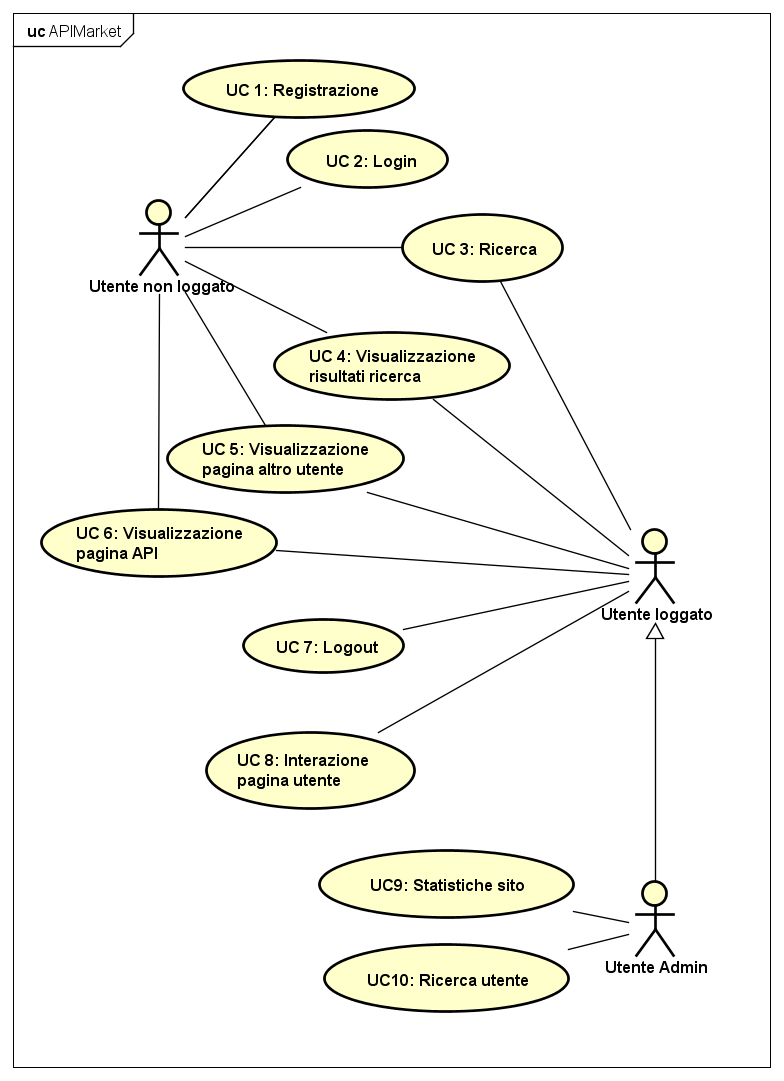
\includegraphics[width=0.7\textwidth]{UseCase/APIMarket}
		\caption{Operazioni ad alto livello}
	\end{figure}
	\begin{itemize}
		\item \textbf{Attori:} Utente non autenticato
		\item \textbf{Scopo e descrizione:} La pagina presenta tutti i servizi che sono offerti ad un utente non autenticato ovvero:
		\begin{itemize} 
			\item Viene offerta la possibilità di registrarsi al market; 
			\item Viene offerta la possibilità di identificarsi se già in possesso di un account all'interno del market;
			\item Viene offerta la possibilità di consultare, solo a scopo informativo, le API all'interno del market (per poter caricare le proprie API, o acquistare APIKey è necessario accedere con il proprio account); 
			\item Viene offerta la possibilità di consultare le statistiche riferite agli utenti all'interno del market;
		\end{itemize}
		\item \textbf{Precondizione:} Il sistema viene avviato da un utente esterno
		\item \textbf{Postcondizione:} Il sistema offre tutti servizi che un utente non autenticato può usufruire
	\end{itemize}
	\subsection{Caso d'uso UC1: Registrazione}
	\label{UC1}
	\begin{figure}[ht]
		\centering
		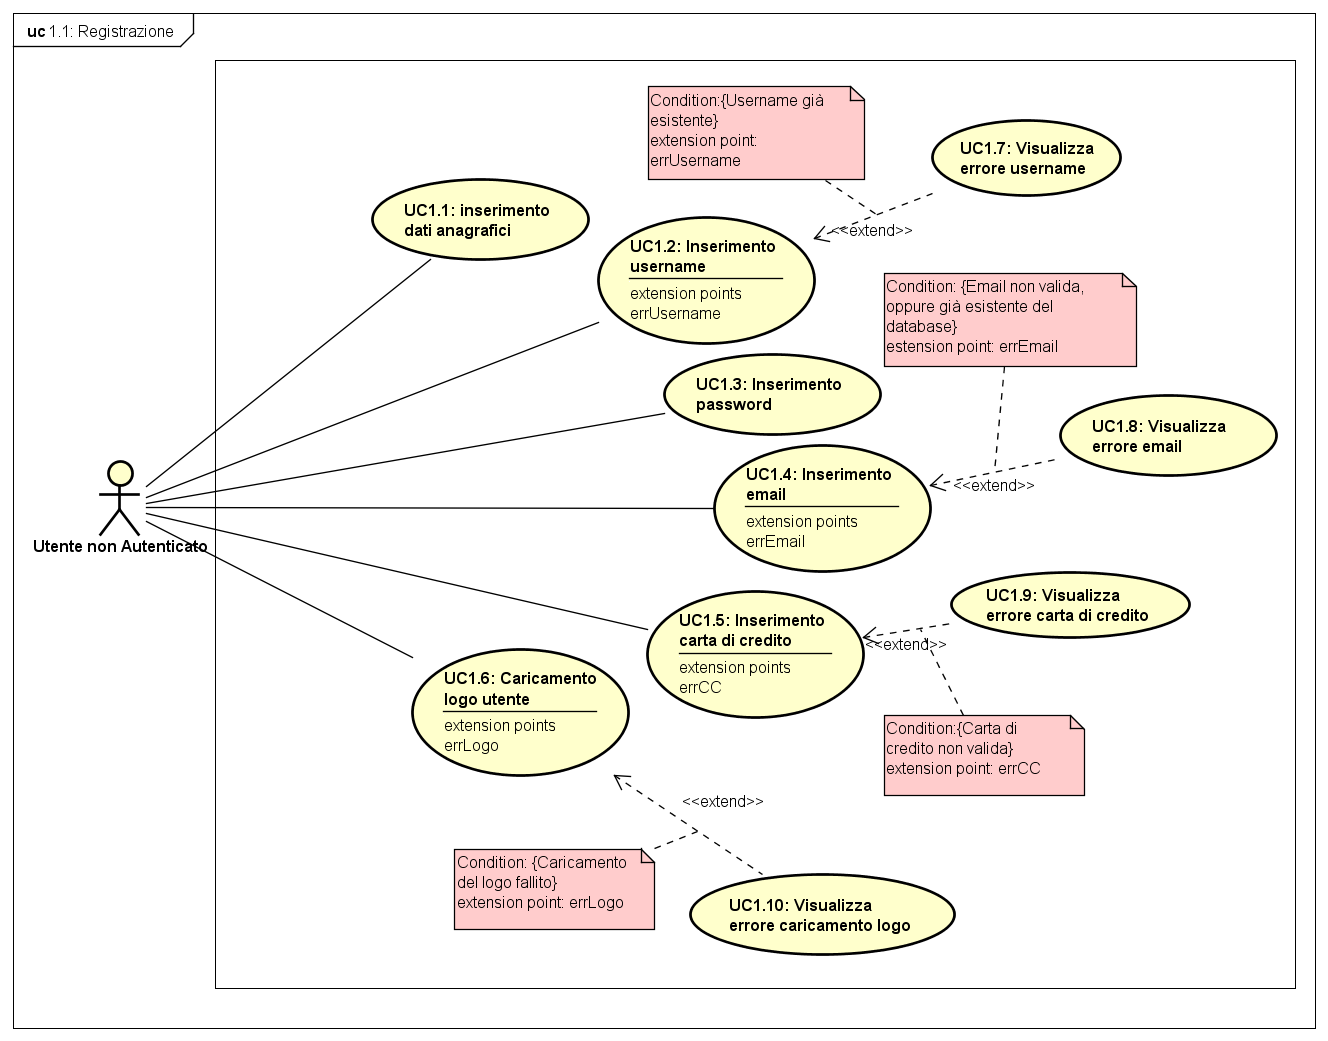
\includegraphics[width=0.8\textwidth]{UseCase/Registrazione}
		\caption{Registrazione}
	\end{figure}
	\begin{itemize}
		\item \textbf{Attori: Utente non autenticato}
		\item \textbf{Scopo e descrizione:} L'utente non in possesso di un username ed una password inserisce i suoi dati anagrafici da associare al nuovo username; gli verrà chiesta anche una password che dovrà utilizzare ogni qual volta debba effettuare l'accesso;
		\item \textbf{Scenari alternativi:} Scenari alternativi: L'inserimento viene annullato per i seguenti motivi:
		\begin{itemize}
			\item username già esistente;
			\item password non soddisfa i criteri esposti. In tal caso viene richiesto all'utente di ripetere l'operazione.
		\end{itemize}
		\item \textbf{Precondizione:} Il sistema attende l'inserimento dei dati richiesti;
		\item \textbf{Postcondizione:} Il sistema ha salvato le informazione date dall'utente e ha mostrato all'utente un messaggio di avvenuta registrazione.
	\end{itemize}
	\subsection{Caso d'uso UC1.1: Inserimento dati anagrafici}
	\label{UC1.1}
	\begin{figure}[ht]
		\centering
		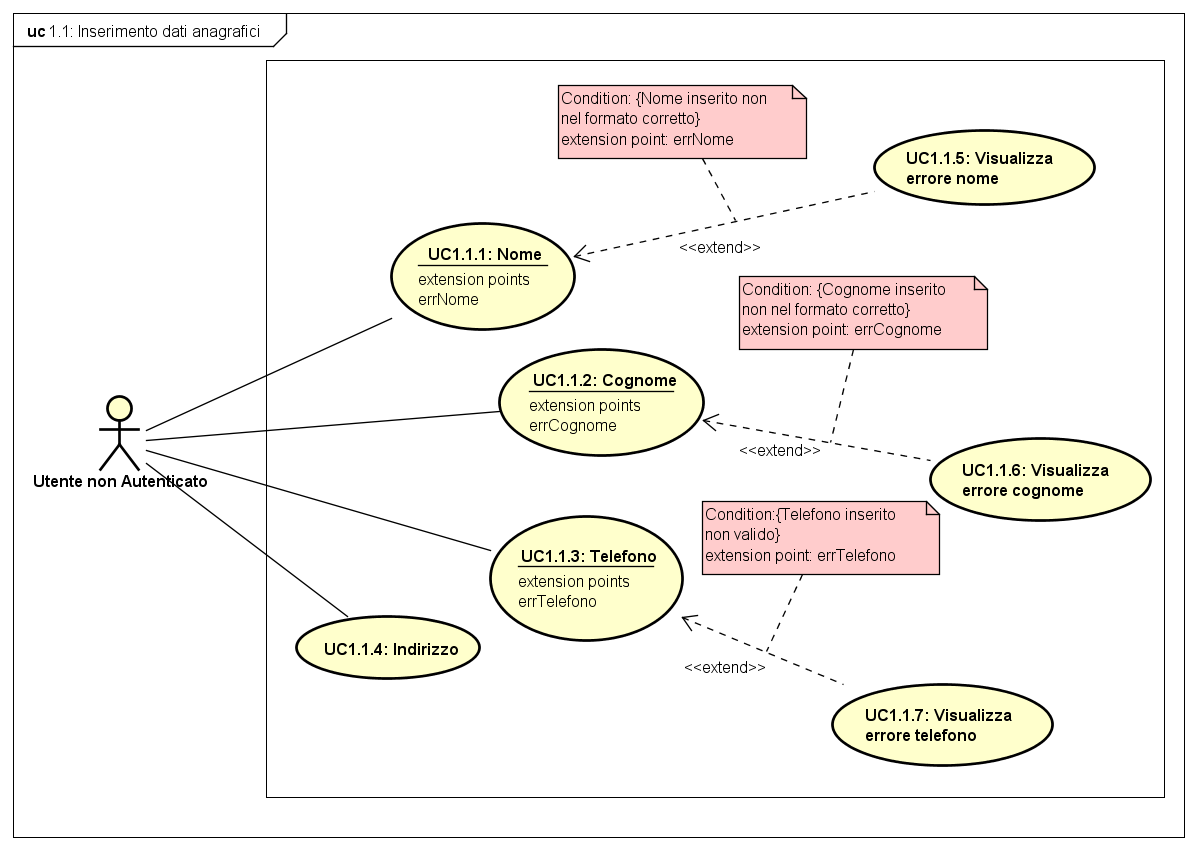
\includegraphics[width=0.7\textwidth]{UseCase/InserimentoDatiAnagrafici}
		\caption{Inserimento dati anagrafici}
	\end{figure}
	\begin{itemize}
		\item \textbf{Attori:} Utente non autenticato;
		\item \textbf{Scopo e descrizione:} L'utente non ancora autenticato inserisce i propri dati anagrafici (nome, cognome, nazionalità);
		\item \textbf{Precondizione:} Il sistema attende l'inserimento dei dati richiesti;
		\item \textbf{Postcondizione:} Il sistema salva le informazione date dall'utente.
	\end{itemize}
	\subsection{Caso d'uso UC1.1.1: Inserimento del nome}
	\label{UC1.1.1}
	\begin{itemize}
		\item \textbf{Attori:} Utente non autenticato; 
		\item \textbf{Scopo e descrizione:} L'utente deve inserire il suo nome;
		\item \textbf{Scenario alternativo:} Il nome inserito dall'utente non è conforme al formato richiesto;
		\item \textbf{Precondizione:} Il sistema attende l'inserimento del nome da parte dell'utente;
		\item \textbf{Postcondizione:} Il sistema inserisce nel DB il nome dell'utente.
	\end{itemize}
	\subsection{Caso d'uso UC1.1.2: Inserimento del cognome}
	\label{UC1.1.2}
	\begin{itemize}
		\item \textbf{Attori:} Utente non autenticato;
		\item \textbf{Scopo e descrizione:} L'utente deve inserire il suo nome;
		\item \textbf{Scenario alternativo:} Il nome inserito dall'utente non è conforme al formato richiesto;
		\item \textbf{Precondizione:} Il sistema attende l'inserimento del nome da parte dell'utente;
		\item \textbf{Postcondizione:} Il sistema inserisce nel DB il nome dell'utente.
	\end{itemize}
	\subsection{Caso d'uso UC1.1.3: Inserimento del telefono}
	\label{UC1.1.3}
	\begin{itemize}
		\item \textbf{Attori:} Utente non autenticato;
		\item \textbf{Scopo e descrizione:} L'utente deve inserire il suo numero di telefono;
		\item \textbf{Scenario alternativo:} Il numero di telefono inserito dall'utente non è valido;
		\item \textbf{Precondizione:} Il sistema attende l'inserimento del numero di telefono da parte dell'utente;
		\item \textbf{Postcondizione:} Il sistema inserisce nel DB il numero di telefono dell'utente.
	\end{itemize}
	\subsection{Caso d'uso UC1.1.4: Inserimento indirizzo}
	\label{UC1.1.4}
	\begin{itemize}
		\item \textbf{Attori:} Utente non autenticato;
		\item \textbf{Scopo e descrizione:} L'utente deve inserire il suo indirizzo per la fatturazione degli acquisti. In particolare deve essere richiesto all'utente:
		\begin{itemize}
			\item Indirizzo;
			\item CAP;
			\item Paese.
		\end{itemize}
		\item \textbf{Precondizione:} Il sistema attende che l'utente inserisca il proprio indirizzo;
		\item \textbf{Postcondizione: }Il sistema inserisce nel DB l'indirizzo dell'utente.
	\end{itemize}
	\subsection{Caso d'uso UC1.1.5: Visualizza errore nome}
	\label{UC1.1.5}
	\begin{itemize}
		\item \textbf{Attori:} Utente non autenticato;
		\item \textbf{Scopo e descrizione:} L'utente ha inserito un nome non valido. Gli viene quindi notificato l'errore;
		\item \textbf{Precondizione:} L'utente ha inserito il nome errato;
		\item \textbf{Postcondizione:} Il sistema ha mostrato all'utente un messaggio di errore appropriato.
	\end{itemize}
	\subsection{Caso d'uso UC1.1.6: Visualizza errore cognome}
	\label{UC1.1.6}
	\begin{itemize}
		\item \textbf{Attori:} Utente non autenticato;
		\item \textbf{Scopo e descrizione:} L'utente ha inserito un cognome non valido. Gli viene quindi notificato l'errore;
		\item \textbf{Precondizione:} L'utente ha inserito il cognome errato;
		\item \textbf{Postcondizione:} Il sistema ha mostrato all'utente un messaggio di errore appropriato.
	\end{itemize}
	\subsection{Caso d'uso UC1.1.7: Visualizza errore telefono}
	\label{UC1.1.7}
	\begin{itemize}
		\item \textbf{Attori:} Utente non autenticato;
		\item \textbf{Scopo e descrizione:} L'utente ha inserito un numero di telefono non valido. Gli viene quindi notificato l'errore;
		\item \textbf{Precondizione:} L'utente ha inserito il numero di telefono errato;
		\item \textbf{Postcondizione:} Il sistema ha mostrato all'utente un messaggio di errore appropriato.
	\end{itemize}
	\subsection{Caso d'uso UC1.2: Inserimento nome utente}
	\label{UC1.2}
	\begin{itemize}
		\item \textbf{Attori: }Utente non autenticato;
		\item \textbf{Scopo e descrizione: }L'utente inserisce lo username che gli servirà ad identificarsi nel sistema nel futuro;
		\item \textbf{Scenario alternativo: }Il sistema rifiuta lo username dato in quanto già presente nel DB, in tal caso viene chiesto di inserire all'utente un diverso username;
		\item \textbf{Precondizione: }Il sistema rimane in attesa dell'inserimento dello username;
		\item \textbf{Postcondizione: }Il sistema associa allo username i dati anagrafici inseriti in precedenza ed inserisce lo username nel DB degli utenti.
	\end{itemize}
	\subsection{Caso d'uso UC1.3: Inserimento password (Registrazione)}
	\label{UC1.3}
	\begin{figure}[H]
		\centering
		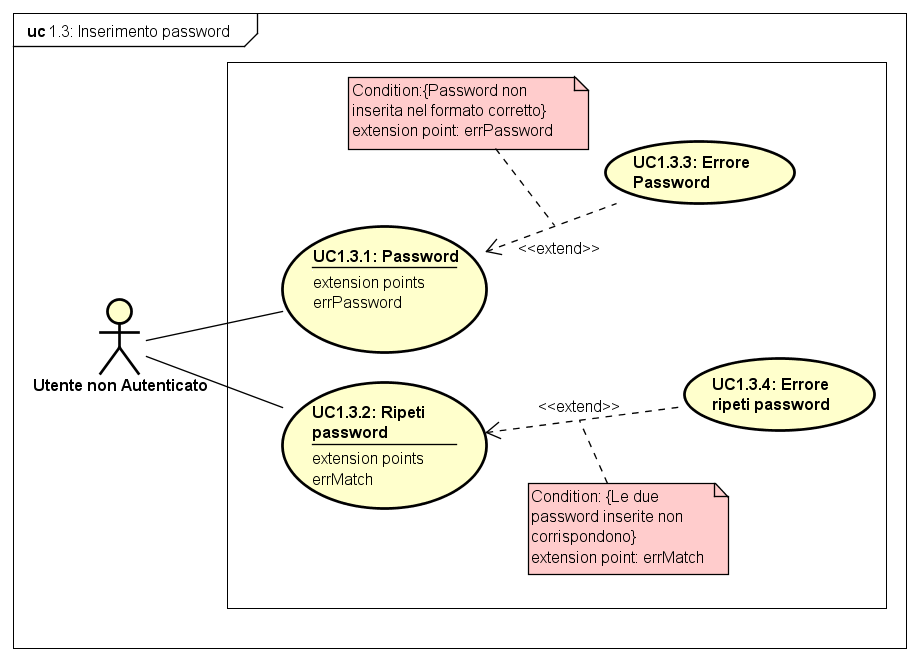
\includegraphics[width=0.7\textwidth]{UseCase/InserimentoPassword}
		\caption{Inserimento password (Registrazione)}
	\end{figure}
	\begin{itemize}
		\item \textbf{Attori: }Utente non autenticato;
		\item \textbf{Scopo e descrizione: } L'utente non autenticato inserisce una password che gli servirà come chiave di sicurezza per identificarsi nel sistema. La password richiesta, per poter essere accettata, deve soddisfare i seguenti requisiti: 
		\begin{itemize}
			\item Essere lunga almeno 8 caratteri; 
			\item Contenere almeno 1 carattere maiuscolo; 
			\item Contere almeno 1 carattere minuscolo;
		\end{itemize}
		Inoltre la password inserita deve essere ripetuta come controllo di sicurezza.
		\item \textbf{Scenario alternativo: }La password inserita dall'utente non è conforme alle richieste, perciò il sistema chiede all'utente di inserire una nuova password che sia conforme, oppure la password ripetuta non combacia.
		\item \textbf{Precondizione: }Il sistema attende che l'utente inserisca la password da associare al suo username;
		\item \textbf{Postcondizione: }Il sistema accetta la password inserita dall'utente e la associa allo username nel DB corrispondente.
	\end{itemize}
	\subsection{Caso d'uso UC1.3.1: Password}
	\label{UC1.3.1}
	\begin{itemize}
		\item \textbf{Attori: }Utente non autenticato;
		\item \textbf{Scopo e descrizione: }L'utente deve inserire la sua password con cui accederà al suo account una volta terminata la registrazione;
		\item \textbf{Scenario alternativo: }La password inserita non rispetta i requisiti minimi, viene quindi mostrato un messaggio d'errore;
		\item \textbf{Precondizione: }L'utente è nella schermata di registrazione e deve inserire la password;
		\item \textbf{Postcondizione: }L'utente ha inserito una password valida.
	\end{itemize}
	\subsection{Caso d'uso UC1.3.2: Ripeti password}
	\label{UC1.3.2}
	\begin{itemize}
		\item \textbf{Attori: }Utente non autenticato;
		\item \textbf{Scopo e descrizione: }L'utente deve reinserire la password come controllo di sicurezza;
		\item \textbf{Scenario alternativo: }L'utente ha inserito una password che non combacia con la password inserita in precedenza, viene quindi mostrato un messaggio di errore;
		\item \textbf{Precondizione: }L'utente è nella schermata di registrazione ed ha inserito la password, deve inserire la password una seconda volta;
		\item \textbf{Postcondizione: }L'utente ha inserito la password per la seconda volta in modo corretto
	\end{itemize}
	\subsection{Caso d'uso UC1.3.3: Errore password}
	\label{UC1.3.3}
	\begin{itemize}
		\item \textbf{Attori: }Utente non autenticato;
		\item \textbf{Scopo e descrizione: }L'utente ha inserito una password che non rispetta gli standard minimi. Il sistema rifiuta la password e mostra all'utente un errore;
		\item \textbf{Precondizione: }L'utente ha inserito la password errata;
		\item \textbf{Postcondizione: }Il sistema ha mostrato all'utente un errore appropriato.
	\end{itemize}
	\subsection{Caso d'uso UC1.3.4: Errore ripeti password}
	\label{UC1.3.4}
	\begin{itemize}
		\item \textbf{Attori: }Utente non autenticato;
		\item \textbf{Scopo e descrizione: }L'utente ha inserito una password che non corrisponde a quella inserita in precedenza. Il sistema notifica all'utente l'errore.
		\item \textbf{Precondizione: }L'utente ha inserito la password di conferma errata;
		\item \textbf{Postcondizione: }Il sistema ha mostrato all'utente un errore appropriato.
	\end{itemize}
	\subsection{Caso d'uso UC1.4: Inserimento email}
	\label{UC1.4}
	\begin{itemize}
		\item \textbf{Attori: }Utente non autenticato;
		\item \textbf{Scopo e descrizione: }In futuro nel caso in cui l'utente si fosse dimenticato la password, è necessario che il sistema abbia a disposizione un'email alla quale fare affidamento a cui poter mandare la password per poter far accedere l'utente;
		\item \textbf{Scenario alternativo: }L'email inserita non è nel formato valido, o esiste già nel database, quindi il sistema chiede all'utente di inserire un'altra email valida;
		\item \textbf{Precondizione: }Il sistema attende una email dall'utente;
		\item \textbf{Postcondizione: }Il sistema riceve una email che assocerà allo username dell'utente.
	\end{itemize}
	\subsection{Caso d'uso UC1.5: Inserimento carta di credito}
	\label{UC1.5}
	\begin{itemize}
		\item \textbf{Attori: }Utente non autenticato;
		\item \textbf{Scopo e descrizione: }L'utente deve disporre di un metodo di una carta di credito valida che gli permetta di effettuare acquisti all'interno del market;
		\item \textbf{Scenario alternativo: }La carta di credito non è valida perciò viene segnalato errore e viene chiesto all'utente di inserirne una diversa;
		\item \textbf{Precondizione: }Il sistema attende che l'utente inserisca una carta di credito valida;
		\item \textbf{Postcondizione: }Il sistema ha validato la carta di credito inserita dall'utente e l'ha associata al suo account.
	\end{itemize}
	\subsection{Caso d'uso UC1.6: Caricamento logo utente}
	\label{UC1.6}
	\begin{itemize}
		\item \textbf{Attori: }Utente non autenticato;
		\item \textbf{Scopo e descrizione: }L'utente può caricare un logo per il suo profilo. Deve corrispondere ai seguenti requisiti:
		\begin{itemize}
			\item La dimensione del file deve essere <500kb;
			\item L'estesione del file deve essere .jpg, .jpeg, .png, .bmp;
		\end{itemize}
		\item \textbf{Scenario alternativo: }Il file è troppo grande o non è in un formato supportato, viene quindi mostrato un messaggio di errore;
		\item \textbf{Precondizione: }Il sistema attende che l'utente carichi un'immagine di logo;
		\item \textbf{Postcondizione: }Il sistema ha controllato che l'immagine sia valida e, se è valida, l'ha caricata e associata al profilo.
	\end{itemize}
	\subsection{Caso d'uso UC1.7: Visualizza errore username}
	\label{UC1.7}
	\begin{itemize}
		\item \textbf{Attori: }Utente non autenticato;
		\item \textbf{Scopo e descrizione: }L'utente ha inserito un username già esistente nel sistema. Viene mostrato un errore che invita l'utente ad inserirne un altro
		\item \textbf{Precondizione: }L'utente ha tentato di creare un account con uno username già esistente;
		\item \textbf{Postcondizione: }Il sistema ha mostrato all'utente un messaggio di errore appropriato.
	\end{itemize}
	\subsection{Caso d'uso UC1.8: Visualizza errore email}
	\label{UC1.8}
	\begin{itemize}
		\item \textbf{Attori: }Utente non autenticato;
		\item \textbf{Scopo e descrizione: }L'utente ha inserito un indirizzo email non valido o già esistente nel database. Gli viene quindi notificato l'errore.
		\item \textbf{Precondizione: }I'utente ha inserito l'indirizzo email errato;
		\item \textbf{Postcondizione: }Il sistema ha mostrato all'utente un messaggio di errore appropriato.
	\end{itemize}
	\subsection{Caso d'uso UC1.9: Visualizza errore carta di credito}
	\label{UC1.9}
	\begin{itemize}
		\item \textbf{Attori: }Utente non autenticato;
		\item \textbf{Scopo e descrizione: }L'utente ha inserito un una carta di credito non valida o già esistente nel database. Gli viene quindi notificato l'errore.
		\item \textbf{Precondizione: }L'utente ha inserito la carta di credito non valida;
		\item \textbf{Postcondizione: }Il sistema ha mostrato all'utente un messaggio di errore appropriato.
	\end{itemize}
	\subsection{Caso d'uso UC1.10: Visualizza errore caricamento logo}
	\label{UC1.10}
	\begin{itemize}
		\item \textbf{Attori: }Utente non autenticato;
		\item \textbf{Scopo e descrizione: }L'utente ha tentato di caricare il suo logo ma il formato non era corretto, il file era troppo grande o il caricamento è fallito. Il sistema mostra all'utente un errore
		\item \textbf{Precondizione: }L'utente ha tentato di caricare il suo logo;
		\item \textbf{Postcondizione: }Il sistema ha mostrato all'utente un messaggio di errore appropriato.
	\end{itemize}
	\subsection{Caso d'uso UC2: Login}
	\label{UC2}
	\begin{figure}[H]
		\centering
		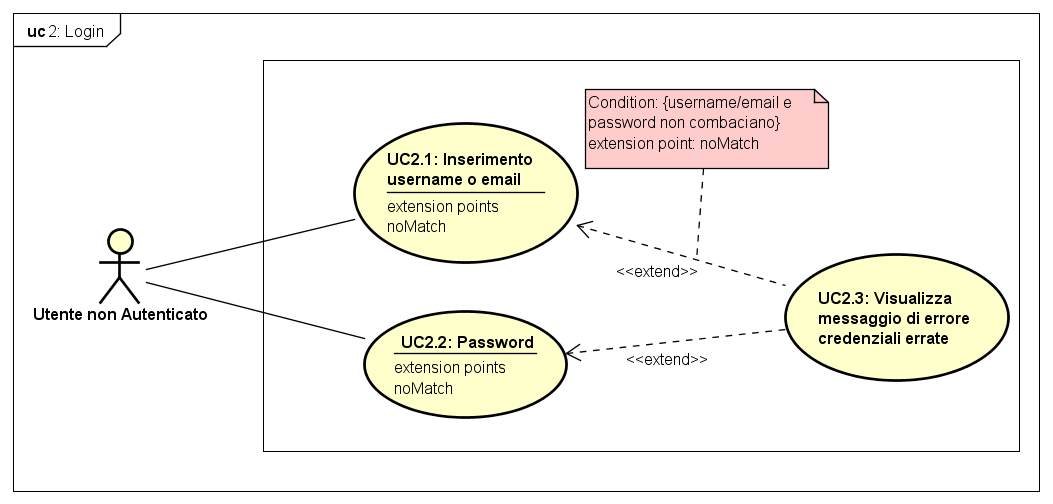
\includegraphics[width=0.7\textwidth]{UseCase/Login}
		\caption{Login}
	\end{figure}
	\begin{itemize}
		\item \textbf{Attori:} Utente non autenticato;
		\item \textbf{Scopo e descrizione:} L'utente che possiede già un username e una password vuole effettuare un accesso;
		\item \textbf{Scenario alternativo: }Il sistema rifiuta l'accesso all'utente a causa di un errato inserimento di username o di password;
		\item \textbf{Precondizione: }Il sistema attende che l'utente inserisca i suoi dati identificativi;
		\item \textbf{Postcondizione: Il sistema ha accettato i dati e manda l'utente alla sua bacheca personale}.
	\end{itemize}
	\subsection{Caso d'uso UC2.1: Inserimento username o email}
	\label{UC2.1}
	\begin{itemize}
		\item \textbf{Attori: }Utente non autenticato;
		\item \textbf{Scopo e descrizione: }Viene chiesto all'utente di inserire il suo username o la sua email per poter essere identificato;
		\item \textbf{Scenario alternativo: }Lo username o l'email non esistono all'interno del DB;
		\item \textbf{Precondizione: }Il sistema attende l'inserimento dello username o dell'email da parte dell'utente;
		\item \textbf{Postcondizione: }Il sistema ha riconosciuto l'utente e attende l'inserimento della password per validare l'accesso.
	\end{itemize}
	\subsection{Caso d'uso UC2.2: Password}
	\label{UC2.2}
	\begin{itemize}
		\item \textbf{Attori: }Utente non autenticato;
		\item \textbf{Scopo e descrizione: }Viene chiesto all'utente di inserire la password associata allo username (o alla relativa email);
		\item \textbf{Scenario alternativo: }La password inserita dall'utente non corrisponde alla password associata allo username perciò viene rifiutato l'accesso;
		\item \textbf{Precondizione: }Il sistema attende l'inserimento della password da parte dell'utente;
		\item \textbf{Postcondizione: }Il sistema ha verificato che la password inserita dall'utente è corretta perciò logga l'utente.
	\end{itemize}
	\subsection{Caso d'uso UC2.3: Visualizza messaggio di errore credenziali errate}
	\label{UC2.3}
	\begin{itemize}
		\item \textbf{Attori: }Utente non autenticato;
		\item \textbf{Scopo e descrizione: }L'utente ha inserito delle credenziali di accesso non corrette. Il sistema quindi non effettua il login e notifica l'errore all'utente;
		\item \textbf{Precondizione: }L'utente ha inserito le credenziali errate;
		\item \textbf{Postcondizione: }Il sistema ha controllato le credenziali ed ha restituito un errore.
	\end{itemize}
	\subsection{Caso d'uso UC2.4: Recupero password}
	\label{UC2.4}
	\begin{itemize}
		\item \textbf{Attori: }Utente non autenticato;
		\item \textbf{Scopo e descrizione: }Nel caso in cui l'utente si fosse dimenticato la password del suo profilo, il sistema offre un'assistenza di recupero password, ovvero invierà alla mail associata al profilo una nuova password temporanea da utilizzare per accedervi e modificarla nuovamente;
		\item \textbf{Precondizione: }Il sistema rimane in attesa della richiesta da parte dell'utente di recuperare la sua password;
		\item \textbf{Postcondizione: }L'utente ha a disposizione una password temporanea che gli permette di accedere al suo profilo e modificarla nuovamente.
	\end{itemize}
	\subsection{Caso d'uso UC3: Ricerca}
	\label{UC3}
	\begin{figure}[H]
		\centering
		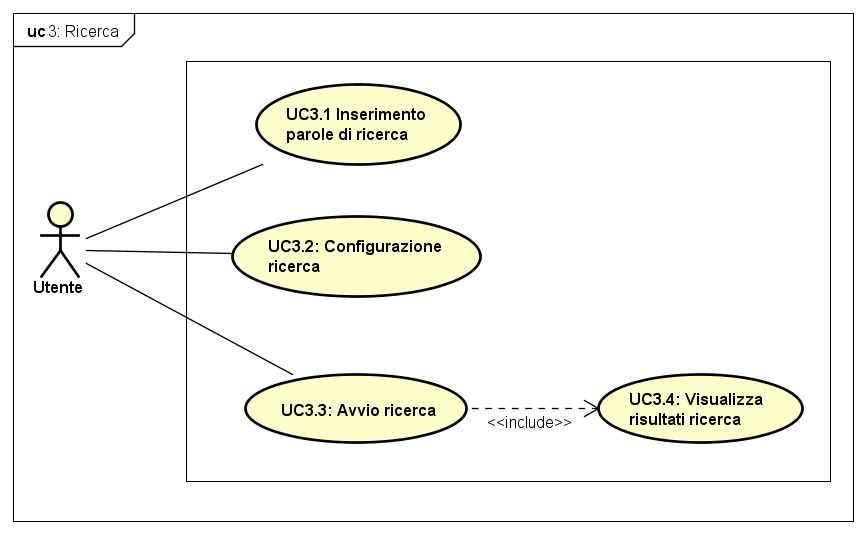
\includegraphics[width=0.7\textwidth]{UseCase/Ricerca}
		\caption{Ricerca}
	\end{figure}
	\begin{itemize}
		\item \textbf{Attori: }Utente non autenticato e Utente autenticato;
		\item \textbf{Scopo e descrizione: }L'utente ricerca nella barra di ricerca il nome di un microservizio e clicca il bottone di conferma;
		\item \textbf{Precondizione: }Il sistema attende l'invio di una frase di ricerca;
		\item \textbf{Postcondizione: }Il sistema ha esaminato la frase di ricerca e restituisce una pagina di risultati della ricerca.
	\end{itemize}
	\subsection{Caso d'uso UC3.1: Inserimento parole di ricerca}
	\label{UC3.1}
	\begin{itemize}
		\item \textbf{Attori: }Utente non autenticato e Utente autenticato;
		\item \textbf{Scopo e descrizione: }L'utente scrive nella barra di ricerca la frase che vuole ricercare;
		\item \textbf{Precondizione: }Il sistema attende l'inserimento di una frase di ricerca;
		\item \textbf{Postcondizione: }L'utente ha terminato di inserire la frase di ricerca.
	\end{itemize}
	\subsection{Caso d'uso UC3.2: Configurazione ricerca}
	\label{UC3.2}
	\begin{figure}[H]
		\centering
		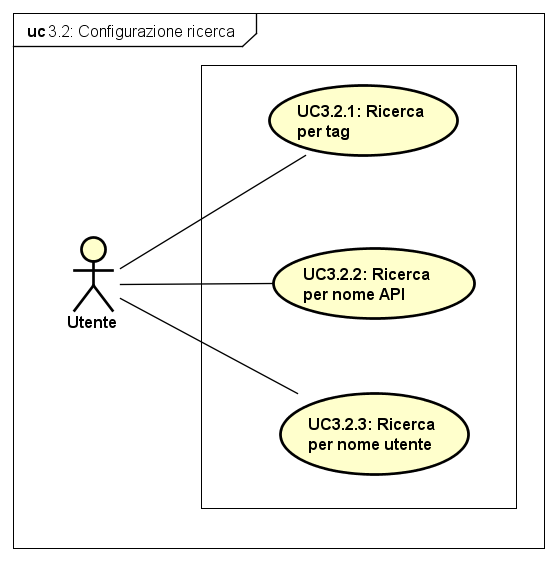
\includegraphics[width=0.7\textwidth]{UseCase/ConfigurazioneRicerca}
		\caption{Configurazione ricerca}
	\end{figure}
	\begin{itemize}
		\item \textbf{Attori: }Utente non autenticato e Utente autenticato;
		\item \textbf{Scopo e descrizione: }L'utente seleziona la modalità con cui vuole eseguire la ricerca;
		\item \textbf{Precondizione: }L'utente non ha ancora scelto nessun metodo di ricerca;
		\item \textbf{Postcondizione: }L'utente ha scelto un metodo di ricerca.
	\end{itemize}
	\subsection{Caso d'uso UC3.2.1: Ricerca per tag}
	\label{UC3.2.1}
	\begin{itemize}
		\item \textbf{Attori: }Utente non autenticato e Utente autenticato;
		\item \textbf{Scopo e descrizione: }L'utente sceglie di cercare all'interno di una categoria precisa di API;
		\item \textbf{Precondizione: }L'utente non ha ancora scelto la configurazione ricerca;
		\item \textbf{Postcondizione: }L'utente ha scelto il tag su cui effettuare la ricerca.
	\end{itemize}
	\subsection{Caso d'uso UC3.2.2: Ricerca per nome API}
	\label{UC3.2.2}
	\begin{itemize}
		\item \textbf{Attori: }Utente non autenticato e Utente autenticato;
		\item \textbf{Scopo e descrizione: }L'utente sceglie di cercare tra tutti i nomi dei microservizi del database;
		\item \textbf{Precondizione: }L'utente non ha ancora scelto la configurazione ricerca;
		\item \textbf{Postcondizione: }L'utente ha scelto la modalità di ricerca per nome API.
	\end{itemize}
	\subsection{Caso d'uso UC3.2.3: Ricerca per nome utente}
	\label{UC3.2.3}
	\begin{itemize}
		\item \textbf{Attori: }Utente non autenticato e Utente autenticato;
		\item \textbf{Scopo e descrizione: }L'utente sceglie di ricercare API tramite il nome utente dell'autore;
		\item \textbf{Precondizione: }L'utente non ha ancora scelto la configurazione ricerca;
		\item \textbf{Postcondizione: }L'utente ha scelto la modalità di ricerca per nome dell'autore.
	\end{itemize}
	\subsection{Caso d'uso UC3.3: Avvio ricerca}
	\label{UC3.3}
	\begin{itemize}
		\item \textbf{Attori: }Utente non autenticato e Utente autenticato;
		\item \textbf{Scopo e descrizione: }L'utente ha impostato la ricerca e preme il tasto per l'avvio della ricerca;
		\item \textbf{Precondizione: }L'utente ha finito di impostare la ricerca;
		\item \textbf{Postcondizione: }L'utente ha avviato la ricerca.
	\end{itemize}
	\subsection{Caso d'uso UC4: Visualizzazione risultati ricerca}
	\label{UC4}
	\begin{itemize}
		\item \textbf{Attori: }Utente non autenticato e Utente autenticato;
		\item \textbf{Scopo e descrizione: }L'utente ha avviato una ricerca e viene reindirizzato alla pagina di visione dei risultati di ricerca. Qui vengono elencate tutti i microservizi attinenti alla sua ricerca, o viene visualizzato un messaggio nel caso la ricerca non abbia prodotto risultati. I risultati devono poter essere ordinati per:
		\begin{itemize}
			\item Pertinenza;
			\item Numero di APIKey vendute;
			\item Valutazione degli utenti;
			\item Data di caricamento.
		\end{itemize}
		\item \textbf{Precondizione: }L'utente ha avviato una ricerca;
		\item \textbf{Postcondizione: }L'utente ha accesso a tutti i microservizi attinenti alla ricerca.
	\end{itemize}
	\subsection{Caso d'uso UC5: Visualizzazione pagina altro utente}
	\label{UC5}
	\begin{figure}[H]
		\centering
		\includegraphics[width=0.8\textwidth]{UseCase/VisualizzazionePaginaAltroUtente}
		\caption{Visualizzazione pagina altro utente}
	\end{figure}
	\begin{itemize}
		\item \textbf{Attori: }Utente non autenticato e Utente Autenticato;
		\item \textbf{Scopo e descrizione: }L'utente è arrivato sulla pagina profilo di un altro utente e ne visiona i dati personali;
		\item \textbf{Precondizione: }L'utente vuole visionare i dati di un utente che ha caricato un microservizio;
		\item \textbf{Postcondizione: }L'utente è sulla pagina utente dell'utente che vuole visionare.
	\end{itemize}
	\subsection{Caso d'uso UC5.1: Visualizza dati utente}
	\label{UC5.1}
	\begin{itemize}
		\item \textbf{Attori: }Utente non autenticato e Utente autenticato;
		\item \textbf{Scopo e descrizione: }L'utente vuole visionare i dati di un utente. In particolare il sistema rende visibile:
		\begin{itemize}
			\item Username;
			\item Indirizzo email.
		\end{itemize}
		\item \textbf{Precondizione: }L'utente si trova nella pagina di un altro utente;
		\item \textbf{Postcondizione: }Il sistema ha stampato su schermo il nome di quell'utente e l'utente l'ha visionato.
	\end{itemize}
	\subsection{Caso d'uso UC5.2: Visualizza commenti scritti}
	\label{UC5.2}
	\begin{itemize}
		\item \textbf{Attori: }Utente non autenticato e Utente autenticato;
		\item \textbf{Scopo e descrizione: }L'utente vuole visionare gli ultimi commenti scritti da un altro utente;
		\item \textbf{Precondizione: }L'utente si trova sulla pagina di un altro utente;
		\item \textbf{Postcondizione: }Il sistema ha mostrato su schermo gli ultimi 30 messaggi scritti dall'utente.
	\end{itemize}
	\subsection{Caso d'uso UC5.3: Visualizza microservizi pubblicati}
	\label{UC5.3}
	\begin{itemize}
		\item \textbf{Attori: }Utente non autenticato e Utente autenticato;
		\item \textbf{Scopo e descrizione: }L'utente vuole visionare i microservizi pubblicati da un dato utente, quindi va sulla sua pagina utente e li visiona;
		\item \textbf{Precondizione: }L'utente è sulla pagina di un altro utente;
		\item \textbf{Postcondizione: }Il sistema ha stampato su schermo una tabella che indica i microservizi rilasciati dall'utente, la data di rilascio, e approssimativamente il numero di download.
	\end{itemize}
	\subsection{Caso d'uso UC5.4: Visualizza indice di affidabilità}
	\label{UC5.4}
	\begin{itemize}
		\item \textbf{Attori: }Utente non autenticato e Utente autenticato;
		\item \textbf{Scopo e descrizione: }L'utente vuole verificare l'attendibilità di un altro utente prima di acquistare un suo microservizio, quindi va sulla sua pagina e legge il suo indice di affidabilità;
		\item \textbf{Precondizione: }L'utente è sulla pagina di un altro utente;
		\item \textbf{Postcondizione: }Il sistema calcola un indice di affidabilità per l'utente basato sulla qualità dei microservizi caricati e sulla loro valutazione da parte degli utenti, e lo stampa su schermo.
	\end{itemize}
	\subsection{Caso d'uso UC5.5: Modifica dati utente (admin)}
	\label{UC5.5}
	\begin{itemize}
		\item \textbf{Attori: }Utente Admin;
		\item \textbf{Scopo e descrizione: }L'utente Admin che visiona la pagina di un altro utente decide di cambiare alcuni dati relativi a quell'utente. In particolare l'Utente admin può modificare:
		\begin{itemize}
			\item Nome e Cognome;
			\item Numero di telefono;
			\item Indirizzo email;
			\item Indirizzo;
			\item Password;
			\item Carta di credito;
			\item Commenti scritti dall'utente;
			\item Microservizi registrati dall'utente.
		\end{itemize}
		\item \textbf{Precondizione: }L'utente Admin è sulla pagina di un altro utente;
		\item \textbf{Postcondizione: }L'utente Admin ha modificato tutto ciò che voleva modificare.
	\end{itemize}
	\subsection{Caso d'uso UC5.6: Visualizza dati utente (admin)}
	\label{UC5.6}
	\begin{itemize}
		\item \textbf{Attori: }Utente Admin;
		\item \textbf{Scopo e descrizione: }L'utente Admin che visiona la pagina di un altro utente vedendo tutti i dati dell'utente. In particolare, oltre a quelli già visti da un semplice Utente >utenticato, un Utente Admin può visualizzare:
		\begin{itemize}
			\item Indirizzo email;
			\item numero di telefono;
			\item indirizzo.
		\end{itemize};
		\item \textbf{Precondizione: }L'utente Admin è sulla pagina di un altro utente;
		\item \textbf{Postcondizione: }L'utente Admin ha modificato tutto ciò che voleva modificare.
	\end{itemize}
	\subsection{Caso d'uso UC6: Visualizzazione pagina API}
	\label{UC6}
	\begin{figure}[H]
		\centering
		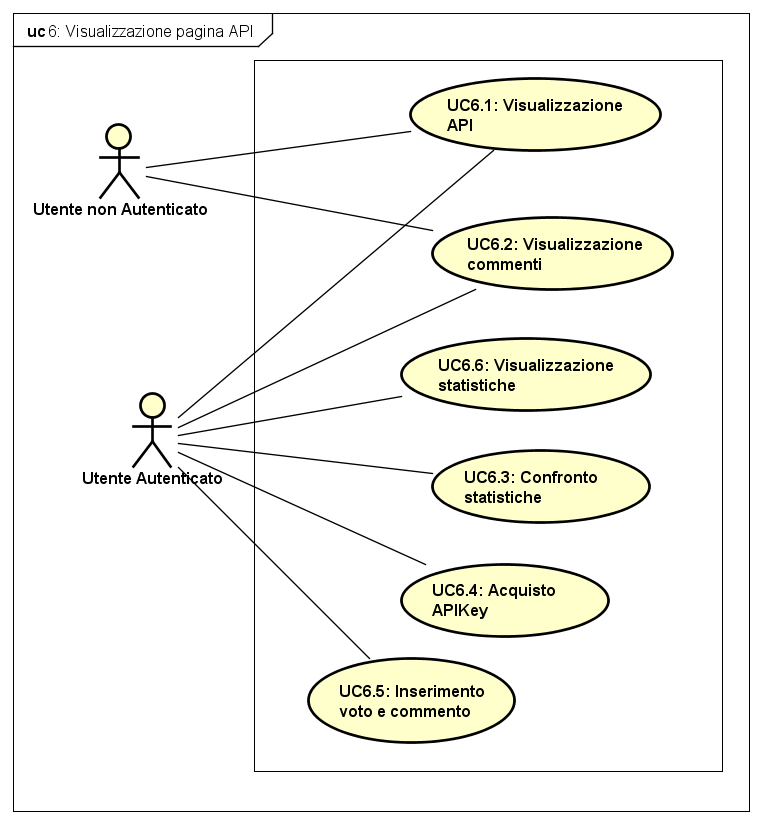
\includegraphics[width=0.8\textwidth]{UseCase/VisualizzazionePaginaAPI}
		\caption{Visualizzazione pagina API}
	\end{figure}
	\begin{itemize}
		\item \textbf{Attori: }Utente non autenticato e Utente autenticato;
		\item \textbf{Scopo e descrizione: }L'utente vuole visionare i dettagli di un microservizio registrato da un utente, apre quindi la pagina relativa a quel microservizio e la legge;
		\item \textbf{Precondizione: }L'utente ha cliccato sul nome di un microservizio;
		\item \textbf{Postcondizione: }L'utente è arrivato alla pagina di un microservizio e il sistema ha caricato tutte le informazioni relative.
	\end{itemize}
	\subsection{Caso d'uso UC 6.1: Visualizzazione API}
	\label{UC6.1}
	\begin{figure}[H]
		\centering
		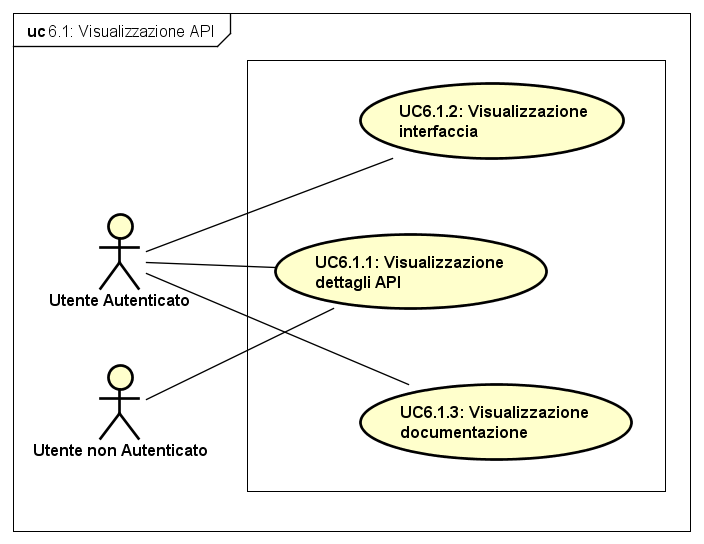
\includegraphics[width=0.7\textwidth]{UseCase/VisualizzazioneAPI}
		\caption{Visualizzazione API}
	\end{figure}
	\begin{itemize}
		\item \textbf{Attori: }Utente non autenticato e Utente autenticato;
		\item \textbf{Scopo e descrizione: }L'utente visualizza le informazioni principali relative al microservizio di cui gli interessano i dettagli;
		\item \textbf{Precondizione: }L'utente è sulla pagina di un microservizio;
		\item \textbf{Postcondizione: }Il sistema mostra all'utente le informazioni base su quel microservizio.
	\end{itemize}
	\subsection{Caso d'uso UC6.1.1: Visualizzazione dettagli API}
	\label{UC6.1.1}
	\begin{itemize}
		\item \textbf{Attori: }Utente non autenticato e Utente Autenticato;
		\item \textbf{Scopo e descrizione: }L'utente legge i dettagli del microservizio nella pagina dedicata. In particolare viene mostrato:
		\begin{itemize}
			\item Nome del microservizio;
			\item Autore del microservizio;
			\item Numero approssimativo di APIKey vendute;
			\item Descrizione del microservizio;
			\item Rating del microservizio dato dai voti degli utenti.
		\end{itemize};
		\item \textbf{Precondizione: }L'utente sta osservando la parte iniziale della pagina relativa ad un microservizio;
		\item \textbf{Postcondizione: }Il sistema ha caricato le informazioni di quel microservizio e le ha stampate a schermo.
	\end{itemize}
	\subsection{Caso d'uso UC6.1.2: Visualizzazione intefaccia}
	\label{UC6.1.2}
	\begin{itemize}
		\item \textbf{Attori: }Utente autenticato;
		\item \textbf{Scopo e descrizione: }L'utente autenticato può visionare l'interfaccia di quel microservizio;
		\item \textbf{Precondizione: }L'utente sta osservando la parte iniziale della pagina relativa ad un microservizio;
		\item \textbf{Postcondizione: }Il sistema ha mostrato all'utente autenticato un link tramite il quale l'utente può osservare il file dell'interfaccia del microservizio.
	\end{itemize}
	\subsection{Caso d'uso UC6.1.3: Visualizzazione documentazione}
	\label{UC6.1.3}
	\begin{itemize}
		\item \textbf{Attori: }Utente autenticato;
		\item \textbf{Scopo e descrizione: }L'utente autenticato può osservare la documentazione relativa ad un microservizio;
		\item \textbf{Precondizione: }L'utente sta osservando la parte iniziale della pagina relativa ad un microservizio;
		\item \textbf{Postcondizione: }Il sistema ha mostrato all'utente autenticato un link tramite il quale l'utente può scaricare la documentazione del microservizio.
	\end{itemize}
	\subsection{Caso d'uso UC6.2: Visualizzazione commenti}
	\label{UC6.2}
	\begin{itemize}
		\item \textbf{Attori: }Utente non autenticato e Utente autenticato;
		\item \textbf{Scopo e descrizione: }L'utente che sta osservando la pagina di un microservizio può leggere i commenti degli altri utenti relativi a quel microservizio;
		\item \textbf{Precondizione: }L'utente è sulla pagina di un microservizio;
		\item \textbf{Postcondizione: }Il sistema mostra a schermo tutti i commenti relativi a quel microservizio, indicando anche il nome dell'autore del commento la data di pubblicazione.
	\end{itemize}
	\subsection{Caso d'uso UC6.3: Confronta statistiche}
	\label{UC6.3}
	\begin{itemize}
		\item \textbf{Attori: }Utente autenticato;
		\item \textbf{Scopo e descrizione: }L'utente autenticato vuole confrontare le statistiche del microservizio con quelle di un altro microservizio. Clicca sul bottone "confronta". Se ha già cliccato su un altro bottone "confronta" in precedenza allora viene reindirizzato ad una pagina in cui vedere il confronto, altrimenti il bottone rimane cliccato in attesa che l'utente prema il bottone "confronta" del microservizio che vuole mettere al confronto.
		\item \textbf{Precondizione: }L'utente sulla pagina di un microservizio clicca sul bottone "confronta";
		\item \textbf{Postcondizione: }Il sistema ha restituito all'utente le statistiche confrontate dei due microservizi scelti, oppure ha mantenuto cliccato il pulsante avvisando l'utente di cliccare sul pulsante "confronta" relativo al microservizio che vuole mettere a confronto.
	\end{itemize}
	\subsection{Caso d'uso UC6.4: Acquisto APIKey}
	\label{UC6.4}
	\begin{itemize}
		\item \textbf{Attori: }Utente autenticato;
		\item \textbf{Scopo e descrizione: }L'utente autenticato vuole acquistare una APIKey, quindi preme sul pulsante di acquisto. Viene reindirizzato nella pagina di conferma di acquisto nel caso abbia un numero di APICredits sufficiente, altrimenti viene condotto nella pagina per l'acquisto di APICredits. Se Ha un numero di APICredits sufficiente e conferma l'acquisto allora il sistema scala gli APICredits dal suo account e gli fornisce una APIKey per quel microservizio.
		\item \textbf{Precondizione: }L'utente autenticato ha cliccato sul pulsante per acquistare una APIKey nella pagina di un microservizio;
		\item \textbf{Postcondizione: }L'utente è in possesso dell'APIKey o è stato condotto nella pagina per l'acquisto di APICredits.
	\end{itemize}
	\subsection{Caso d'uso UC6.5: Inserimento voto e commento}
	\label{UC6.5}
	\begin{itemize}
		\item \textbf{Attori: }Utente autenticato;
		\item \textbf{Scopo e descrizione: }L'utente autenticato che ha acquistato una APIKey relativa al microservizio può rilasciare un commento e una valutazione che va da 1 a 5, e una volta scritto clicca sul pulsante di conferma;
		\item \textbf{Precondizione: }L'utente è sulla pagina di un microservizio;
		\item \textbf{Postcondizione: }Il sistema ricarica la pagina e aggiunge il nuovo commento.
	\end{itemize}
	\subsection{Caso d'uso UC6.6: Visualizzazione statistiche }
	\label{UC6.6}
	\begin{itemize}
		\item \textbf{Attori: }Utente autenticato;
		\item \textbf{Scopo e descrizione: }L'utente vuole visualizzare le statistiche prestazionali di un microservizio, quindi clicca sul link apposito. Viene visualizzata una pagina con le statistiche cercate. In particolare viene mostrato:
		\begin{itemize}
			\item Tempo medio di risposta;
			\item Dati medi scambiati mensilmente;
			\item Numero medio di chiamate mensili.
		\end{itemize}
		\item \textbf{Precondizione: }L'utente è sulla pagina di un microservizio e clicca sul link di visione delle statistiche;
		\item \textbf{Postcondizione: }L'utente è stato reindirizzato alla pagina di visione delle statistiche del microservizio.
	\end{itemize}
	\subsection{Caso d'uso UC7: Logout}
	\label{UC7}
	\begin{itemize}
		\item \textbf{Attori: }Utente autenticato;
		\item \textbf{Scopo e descrizione: }L'utente ha la possibilità di disconnetere il suo profilo dal sistema;
		\item \textbf{Precondizione: }L'utente ha acceduto alla sessione del sistema;
		\item \textbf{Postcondizione: }Il sistema ha disconnesso l'utente dalla sessione a cui apparteneva.
	\end{itemize}
	\subsection{Caso d'uso UC8: Interazione pagina utente}
	\label{UC8}
	\begin{figure}[H]
		\centering
		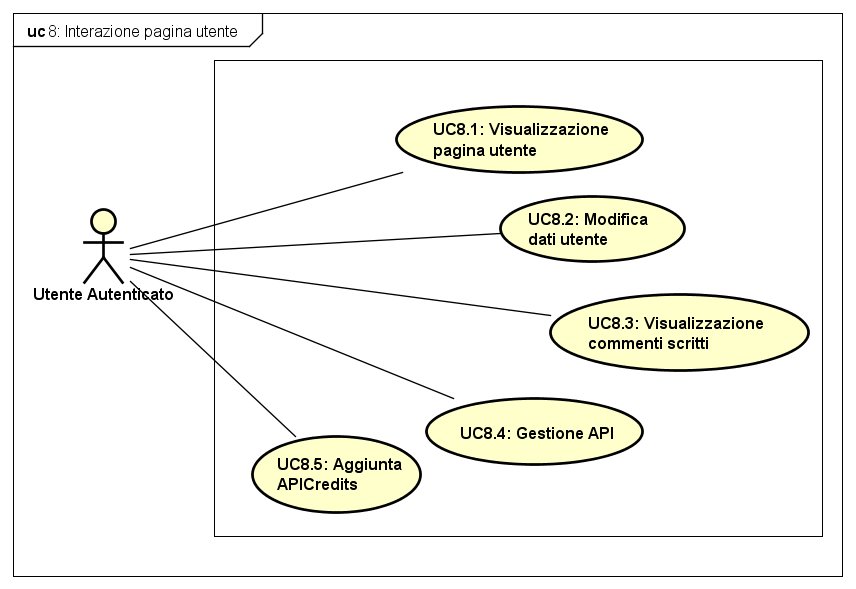
\includegraphics[width=0.7\textwidth]{UseCase/InterazionePaginaUtente}
		\caption{Interazione pagina utente}
	\end{figure}
	\begin{itemize}
		\item \textbf{Attori: }Utente autenticato;
		\item \textbf{Scopo e descrizione: }Un utente autenticato può visitare la sua pagina profilo per visualizzare i suoi dati, modificarli, visionare i suoi commenti scritti, registrare nuovi microservizi e vedere le loro statistiche;
		\item \textbf{Precondizione: }L'utente clicca sul suo profilo;
		\item \textbf{Postcondizione: }Il sistema apre la sua pagina utente.
	\end{itemize}
	\subsection{Caso d'uso UC 8.1: Visualizzazione pagina utente}
	\label{UC8.1}
	\begin{itemize}
		\item \textbf{Attori: }Utente autenticato;
		\item \textbf{Scopo e descrizione: }L'utente sulla sua pagina profilo può visionare tutti i suoi dati inseriti al momento della registrazione. In particolare può visualizzare:
		\begin{itemize}
			\item Nome utente;
			\item Nome e cognome;
			\item Indirizzo email;
			\item Numero di telefono;
			\item Paese di provenienza;
			\item Indice di affidabilità;
			\item APICredits in suo possesso;
			\item La lista delle APIKey acquistate e la loro scadenza.
		\end{itemize}
		\item \textbf{Precondizione: }L'utente è sulla sua pagina profilo;
		\item \textbf{Postcondizione: }Il sistema stampa su schermo tutte le informazioni personali dell'utente.
	\end{itemize}
	\subsection{Caso d'uso UC8.2: Modifica dati utente}
	\label{UC8.2}
	\begin{figure}[H]
		\centering
		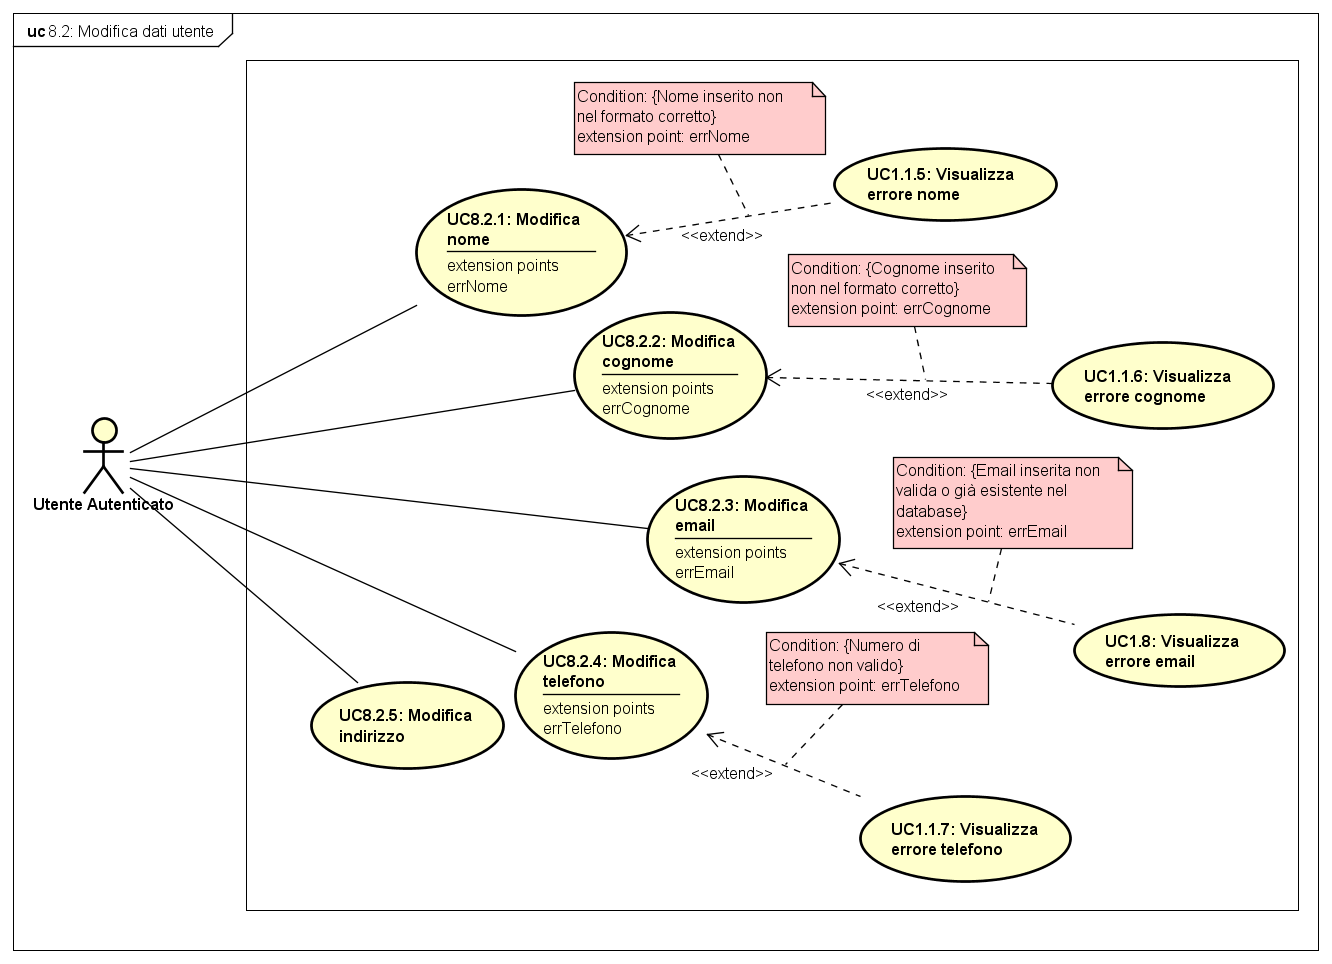
\includegraphics[width=0.8\textwidth]{UseCase/ModificaDatiUtente}
		\caption{Modifica dati utente}
	\end{figure}
	\begin{itemize}
		\item \textbf{Attori: }Utente autenticato;
		\item \textbf{Scopo e descrizione: }L'utente autenticato può modificare tutti i suoi dati ad eccezione del nome utente;
		\item \textbf{Precondizione: }L'utente è sulla sua pagina di profilo e clicca sul pulsante per la modifica dei suoi dati;
		\item \textbf{Postcondizione: }Il sistema ha permesso la modifica dei suoi dati.
	\end{itemize}
	\subsection{Caso d'uso UC8.2.1: Modifica nome}
	\label{UC8.2.1}
	\begin{itemize}
		\item \textbf{Attori: }Utente autenticato;
		\item \textbf{Scopo e descrizione: }L'utente autenticato può modificare il suo nome;
		\item \textbf{Scenario alternativo: }Il nome inserito non è nel formato corretto, il sistema quindi fornisce un errore all'utente;
		\item \textbf{Precondizione: }L'utente è sulla sua pagina utente ed ha cliccato il pulsante per la modifica dei suoi dati;
		\item \textbf{Postcondizione: }L'utente ha modificato i suoi dati.
	\end{itemize}
	\subsection{Caso d'uso UC8.2.2: Modifica cognome}
	\label{UC8.2.2}
	\begin{itemize}
		\item \textbf{Attori: }Utente autenticato;
		\item \textbf{Scopo e descrizione: }L'utente autenticato può modificare il suo cognome;
		\item \textbf{Scenario alternativo: }Il cognome inserito non è nel formato corretto, il sistema quindi fornisce un errore all'utente;
		\item \textbf{Precondizione: }L'utente è sulla sua pagina utente ed ha cliccato il pulsante per la modifica dei suoi dati;
		\item \textbf{Postcondizione: }L'utente ha modificato i suoi dati.
	\end{itemize}
	\subsection{Caso d'uso UC8.2.3: Modifica email}
	\label{UC8.2.3}
	\begin{itemize}
		\item \textbf{Attori: }Utente autenticato;
		\item \textbf{Scopo e descrizione: }L'utente autenticato può modificare il suo indirizzo email;
		\item \textbf{Scenario alternativo: }L'indirizzo email inserito non è nel formato corretto o esiste già nel database, il sistema quindi fornisce un errore all'utente;
		\item \textbf{Precondizione: }L'utente è sulla sua pagina utente ed ha cliccato il pulsante per la modifica dei suoi dati;
		\item \textbf{Postcondizione: }L'utente ha modificato i suoi dati.
	\end{itemize}
	\subsection{Caso d'uso UC8.2.4: Modifica telefono}
	\label{UC8.2.4}
	\begin{itemize}
		\item \textbf{Attori: }Utente autenticato;
		\item \textbf{Scopo e descrizione: }L'utente autenticato può modificare il suo numero di telefono;
		\item \textbf{Scenario alternativo: }Il numero di telefono inserito non è nel formato corretto, il sistema quindi fornisce un errore all'utente;
		\item \textbf{Precondizione: }L'utente è sulla sua pagina utente ed ha cliccato il pulsante per la modifica dei suoi dati;
		\item \textbf{Postcondizione: }L'utente ha modificato i suoi dati.
	\end{itemize}
	\subsection{Caso d'uso UC8.2.5: Modifica indirizzo}
	\label{UC8.2.5}
	\begin{itemize}
		\item \textbf{Attori: }Utente autenticato;
		\item \textbf{Scopo e descrizione: }L'utente autenticato può modificare il suo indirizzo;
		\item \textbf{Precondizione: }L'utente è sulla sua pagina utente ed ha cliccato il pulsante per la modifica dei suoi dati;
		\item \textbf{Postcondizione: }L'utente ha modificato i suoi dati.
	\end{itemize}
	\subsection{Caso d'uso UC8.3: Visualizza commenti scritti}
	\label{UC8.3}
	\begin{itemize}
		\item \textbf{Attori: }Utente autenticato;
		\item \textbf{Scopo e descrizione: }L'utente autenticato visionando il suo profilo può leggere i commenti che ha scritto;
		\item \textbf{Precondizione: }L'utente è sulla sua pagina profilo;
		\item \textbf{Postcondizione: }Il sistema ha stampato su schermo tutti i commenti scritti dall'utente.
	\end{itemize}
	\subsection{Caso d'uso: UC8.4 Gestione API}
	\label{UC8.4}
	\begin{figure}[H]
		\centering
		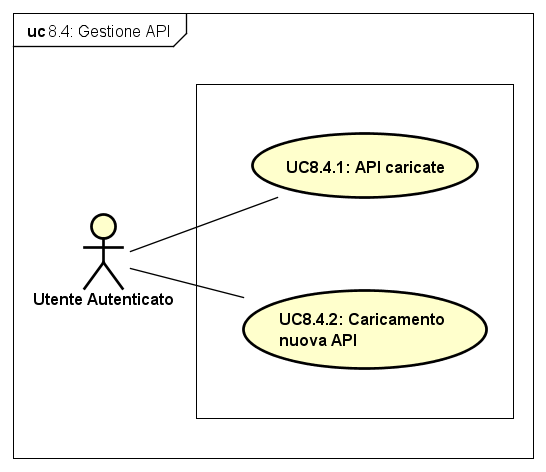
\includegraphics[width=0.5\textwidth]{UseCase/GestioneAPI}
		\caption{Gestione API}
	\end{figure}
	\begin{itemize}
		\item \textbf{Attori: }Utente autenticato;
		\item \textbf{Scopo e descrizione: }L'utente autenticato che visiona il suo profilo ha accesso ad una pagina in cui sono elencate tutti i microservizi da lui registrati, e per ciascuno di essi statistiche che descrivano le sue attività. Può inoltre registrare nuovi microservizi;
		\item \textbf{Precondizione: }L'utente è sulla sua pagina profilo;
		\item \textbf{Postcondizione: }Il sistema ha mostrato all'utente tutte le informazioni sui microservizi da lui caricati, e gli ha permesso di registrare i microservizi che voleva registrare.
	\end{itemize}
	\subsection{Caso d'uso UC8.4.1: Visualizzazione API caricate}
	\label{UC8.4.1}
	\begin{figure}[H]
		\centering
		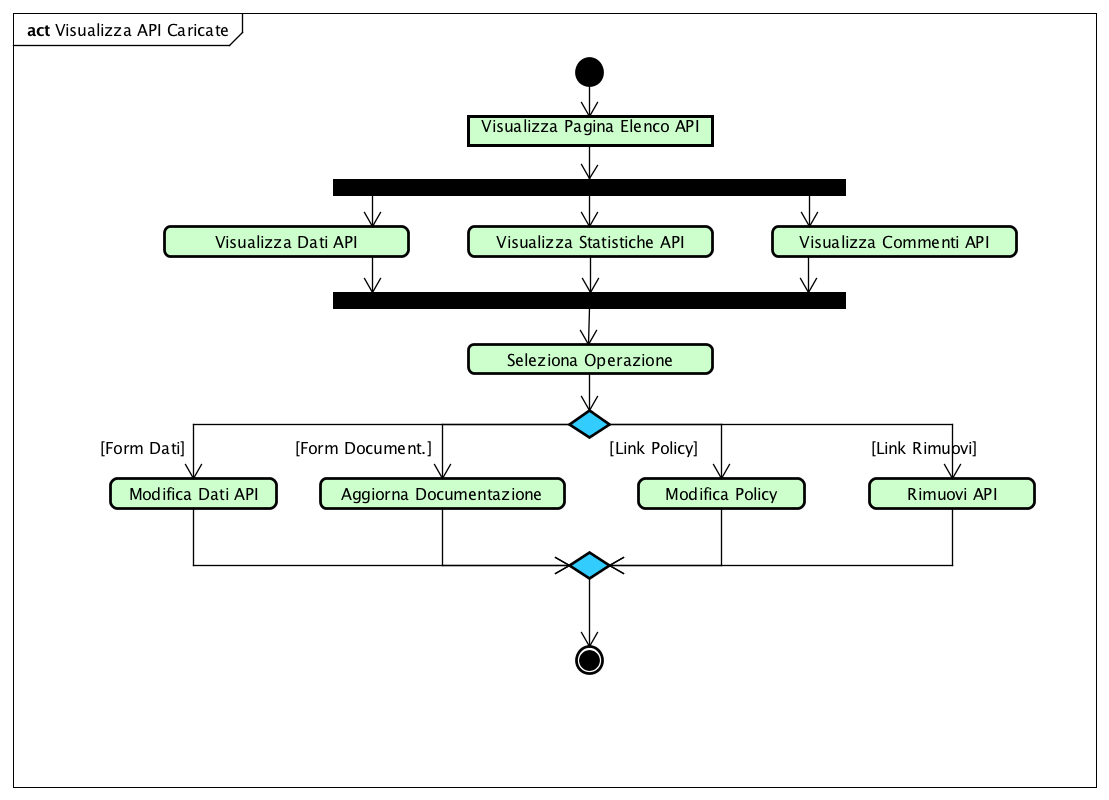
\includegraphics[width=0.5\textwidth]{UseCase/VisualizzaAPICaricate}
		\caption{Visualizza API caricate}
	\end{figure}
	\begin{itemize}
		\item \textbf{Attori: }Utente autenticato;
		\item \textbf{Scopo e descrizione: }L'utente autenticato nella sua pagina utente può visionare tutti i microservizi;
		\item \textbf{Precondizione: }L'utente è sulla sua pagina profilo;
		\item \textbf{Postcondizione: }Il sistema ha mostrato all'utente tutti i microservizi da lui registrati.
	\end{itemize}
	\subsection{Caso d'uso UC8.4.1.1: Visualizza Statistiche API}
	\label{UC8.4.1.1}
	\begin{itemize}
		\item \textbf{Attori: }Utente autenticato;
		\item \textbf{Scopo e descrizione: }L'utente può visionare tutte le statistiche relative ad un particolare microservizio che ha registrato. In particolare:
		\begin{itemize}
			\item Numero di APIKey vendute;
			\item Il guadagno totalo prodotto dal microservizio;
			\item Il guadagno medio mensile prodotto dal microservizio;
			\item L'elenco degli utenti in possesso di una APIKey relativa al microservizio;
			\item Il traffico totale prodotto dal microservizio attraverso l'API Gateway;
			\item Il traffico medio mensile prodotto dal microservizio attraverso l'API Gateway;
			\item L'indice di valutazione degli utenti relativo al microservizio;
			\item L'elenco di tutti commenti degli utenti relativi al microservizio;
			\item L'elenco dei crash commessi dal suo microservizio e notificati dall'API Gateway;
			\item Il tempo medio di risposta al netto del tempo di risposta dell'API Gateway;
			\item Il numero di chiamate totali al microservizio tramite APIKeys;
			\item il numero di chiamate medio mensile al microservizio tramite APIKeys.
		\end{itemize}
		\item \textbf{Precondizione: }L'utente è sulla sua pagina utente ed ha visionato tutti i suoi microservizi registrati;
		\item \textbf{Postcondizione: }Il sistema ha fornito all'utente tutte le statistiche relative al microservizio che interessa all'utente.
	\end{itemize}
	\subsection{Caso d'uso UC8.4.1.2: Modifica API}
	\label{UC8.4.1.2}
	\begin{itemize}
		\item \textbf{Attori: }Utente autenticato;
		\item \textbf{Scopo e descrizione: }L'utente può modificare le informazioni di un microservizio da lui registrato. In particolare può:
		\begin{itemize}
			\item Modificare la descrizione;
			\item Modificare l'interfaccia caricata;
			\item Modificare il prezzo delle APIKey e relative policy di vendita;
			\item Modificare la documentazione relativa.
		\end{itemize}
		\item \textbf{Precondizione: }L'utente sta visionando un microservizio che ha registrato e clicca sul pulsante di modifica dati;
		\item \textbf{Postcondizione: }Il sistema ha permesso all'utente di compiere le modifiche richieste.
	\end{itemize}
	\subsection{Caso d'uso UC8.4.2: Caricamento nuova API}
	\label{UC8.4.2}
	\begin{figure}[H]
		\centering
		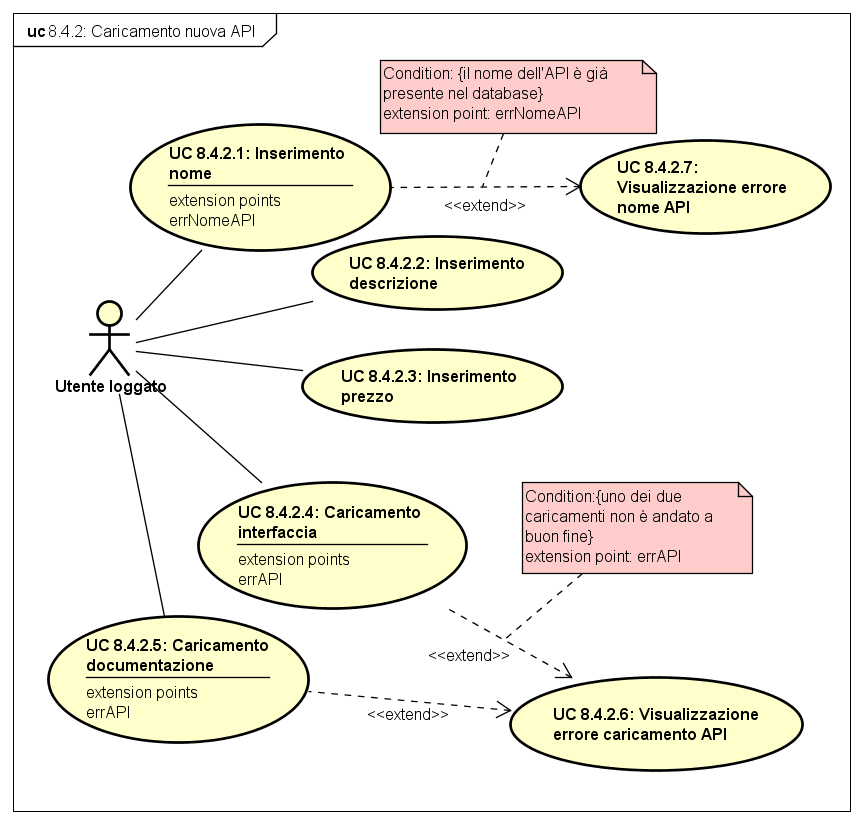
\includegraphics[width=0.7\textwidth]{UseCase/CaricamentoNuovaAPI}
		\caption{Caricamento nuova API}
	\end{figure}
	\begin{itemize}
		\item \textbf{Attori: }Utente autenticato;
		\item \textbf{Scopo e descrizione: }L'utente registrato che vuole registrare una nuova interfaccia di microservizio;
		\item \textbf{Precondizione: }L'utente è sulla sua pagina profilo e ha cliccato sul pulsante per caricare un nuovo microservizio;
		\item \textbf{Postcondizione: }Il sistema ha permesso all'utente di caricare un nuovo microservizio e ha notificato il risultato dell'operazione.
	\end{itemize}
	\subsection{Caso d'uso UC8.4.2.1: Inserimento nome}
	\label{UC8.4.2.1}
	\begin{itemize}
		\item \textbf{Attori: }Utente autenticato;
		\item \textbf{Scopo e descrizione: }L'utente che vuole caricare un microservizio deve inserire un nome per il suo microservizio che sia univoco all'interno del database di APIMarket;
		\item \textbf{Scenario alternativo: }Il nome scelto dall'utente esiste già nel database. Viene notificato all'utente l'errore;
		\item \textbf{Precondizione: }L'utente è nella pagina di registrazione di una nuova interfaccia di microservizio;
		\item \textbf{Postcondizione: }Il sistema ha permesso all'utente di inserire un nome adeguato per il suo microservizio.
	\end{itemize}
	\subsection{Caso d'uso UC8.4.2.2: Inserimento descrizione}
	\label{UC8.4.2.2}
	\begin{itemize}
		\item \textbf{Attori: }Utente autenticato;
		\item \textbf{Scopo e descrizione: }L'utente che vuole caricare un microservizio deve scrivere una descrizione che ne descriva lo scopo generale. Deve inoltre scrivere alcuni tag che categorizzino il suo microservizio e descrivano il suo scopo. Può scrivere da un minimo di tre ad un massimo di dieci tag.
		\item \textbf{Precondizione: }L'utente è nella pagina di registrazione di una nuova interfaccia di microservizio;
		\item \textbf{Postcondizione: }Il sistema ha permesso all'utente di inserire una descrizione per il suo microservizio.
	\end{itemize}
	\subsection{Caso d'uso UC8.4.2.3: Inserimento prezzi}
	\label{UC8.4.2.3}
	\begin{itemize}
		\item \textbf{Attori: }Utente autenticato;
		\item \textbf{Scopo e descrizione: }L'utente che vuole caricare un microservizio deve inserire tutte le modalità di pagamento che desidera impostare. In particolare deve essere possibile per l'utente selezionare le seguenti policy di vendita e il relativo costo:
		\begin{itemize}
			\item A scambio di dati;
			\item A numero di accessi
			\item A scadenza.
		\end{itemize} 
		\item \textbf{Precondizione: }L'utente è nella pagina di registrazione di una nuova interfaccia di microservizio;
		\item \textbf{Postcondizione: }Il sistema ha permesso all'utente di inserire le modalità di pagamento per il suo microservizio.
	\end{itemize}
	\subsection{Caso d'uso UC8.4.2.4: Caricamento interfaccia}
	\label{UC8.4.2.4}
	\begin{itemize}
		\item \textbf{Attori: }Utente Autenticato;
		\item \textbf{Scopo e descrizione: }L'utente che vuole caricare un microservizio deve caricare la sua interfaccia;
		\item \textbf{Scenario alternativo: }Il caricamento dell'interfaccia non è andato a buon fine. Viene notificato all'utente l'errore;
		\item \textbf{Precondizione: }L'utente è nella pagina di registrazione di una nuova interfaccia di microservizio;
		\item \textbf{Postcondizione: }Il sistema ha permesso all'utente di caricare l'interfaccia del suo microservizio.
	\end{itemize}
	\subsection{Caso d'uso UC8.4.2.5: Caricamento documentazione}
	\label{UC8.4.2.5}
	\begin{itemize}
		\item \textbf{Attori: }Utente Autenticato;
		\item \textbf{Scopo e descrizione: }L'utente che vuole caricare un microservizio deve caricare la sua documentazione;
		\item \textbf{Scenario alternativo: }Il caricamento dell'interfaccia non è andato a buon fine. Viene notificato all'utente l'errore;
		\item \textbf{Precondizione: }L'utente è nella pagina di registrazione di una nuova interfaccia di microservizio;
		\item \textbf{Postcondizione: }Il sistema ha permesso all'utente di caricare la documentazione del suo microservizio.
	\end{itemize}
	\subsection{Caso d'uso UC8.4.2.6: Visualizzazione errore caricamento API}
	\label{UC8.4.2.6}
	\begin{itemize}
		\item \textbf{Attori: }Utente Autenticato;
		\item \textbf{Scopo e descrizione: }L'utente ha caricato l'interfaccia e la documentazione ma il caricamento non è andato a buon fine. Il sistema notifica un errore;
		\item \textbf{Precondizione: }L'utente ha tentato di caricare interfaccia e documentazione del suo microservizio
		\item \textbf{Postcondizione: }Il sistema ha notificato all'utente un errore adeguato.
	\end{itemize}
	\subsection{Caso d'uso UC8.4.2.7: Visualizzazione errore nome API}
	\label{UC8.4.2.7}
	\begin{itemize}
		\item \textbf{Attori: }Utente Autenticato;
		\item \textbf{Scopo e descrizione: }L'utente tenta di nominare un suo microservizio con un nome già esistente nel database. Il sistema notifica un errore;
		\item \textbf{Precondizione: }L'utente ha inserito un nome per il suo microservizio già esistente nel database;
		\item \textbf{Postcondizione: }Il sistema ha fallito nel caricamento e ha notificato un errore adeguato all'utente.
	\end{itemize}
	\subsection{Caso d'uso UC8.5: Aggiunta APICredits}
	\label{UC8.4.5}
	\begin{itemize}
		\begin{figure}[H]
			\centering
			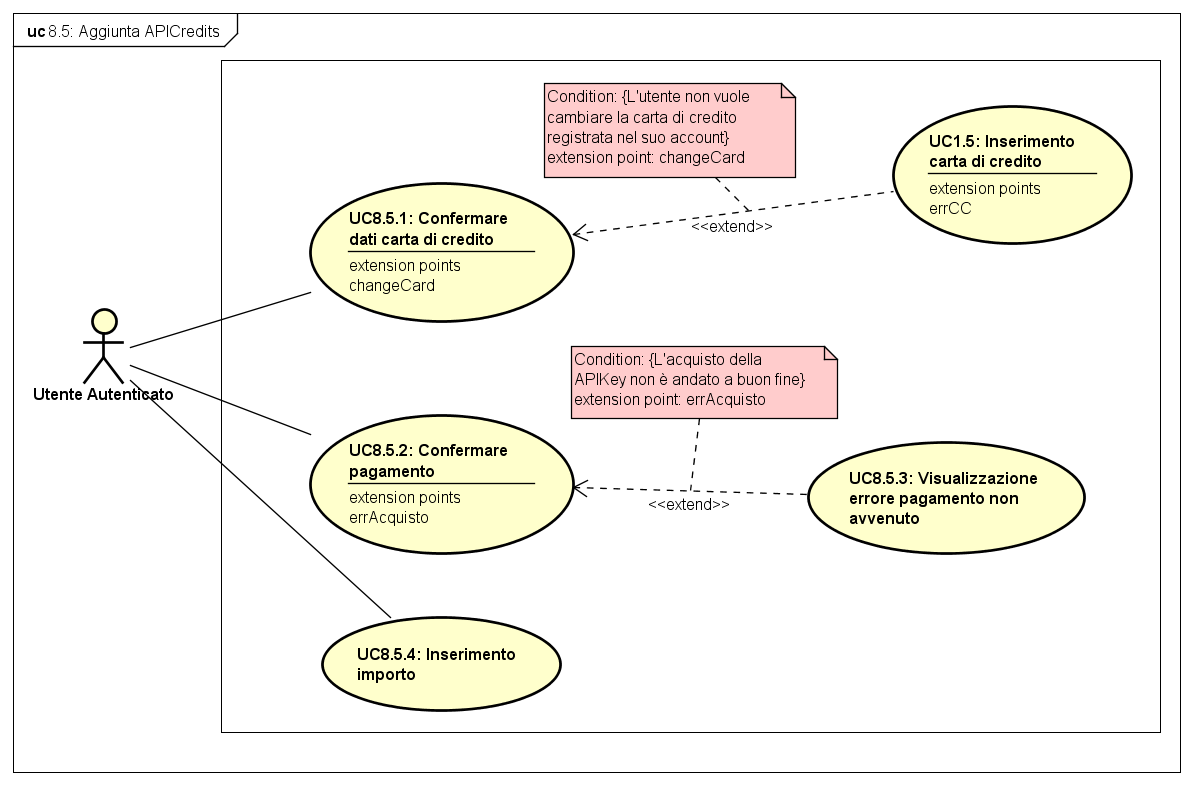
\includegraphics[width=0.8\textwidth]{UseCase/AggiuntaAPICredits}
			\caption{Caricamento nuova API}
		\end{figure}
		\item \textbf{Attori: }Utente Autenticato;
		\item \textbf{Scopo e descrizione: }L'utente può decidere di aggiungere al suo profilo APICredits, la moneta virtuale per comprare API. Viene rediretto su una pagina dove può inserire in numero di APICredits che desidera acquistare e può completare la transazione;
		\item \textbf{Precondizione: }L'utente clicca sul pulsante per aggiungere APICredits;
		\item \textbf{Postcondizione: }Il sistema redirige l'utente nella pagina di acquisto e accompagna l'utente fino ad acquisto ultimato.
	\end{itemize}
	\subsection{Caso d'uso UC8.5.1: Confermare carta di credito}
	\label{UC8.5.1}
	\begin{itemize}
		\item \textbf{Attori: }Utente autenticato;
		\item \textbf{Scopo e descrizione: }L'utente decide se confermare la sua carta di credito registrata nel suo account o se cambiarla;
		\item \textbf{Scenario alternativo: }L'utente decide di cambiare la carta di credito con cui effettuare l'acquisto, viene quindi reindirizzato ad una pagina in cui inserire una carta di credito.
		\item \textbf{Precondizione: }L'utente è nella pagina di conferma di acquisto;
		\item \textbf{Postcondizione: }L'utente ha una carta di credito valida con cui effettuare il pagamento.
	\end{itemize}
	\subsection{Caso d'uso UC8.5.2: Confermare pagamento}
	\label{UC8.5.2}
	\begin{itemize}
		\item \textbf{Attori: }Utente autenticato;
		\item \textbf{Scopo e descrizione: }L'utente conferma il pagamento cliccando sul pulsante di conferma, viene reindirizzato su una pagina che annuncia l'esito dell'operazione e, se l'operazione è andata a buon fine, visualizza la sua nuova APIkey;
		\item \textbf{Scenario alternativo: }L'operazione non va a buon fine, viene quindi visualizzato un messaggio di errore transazione non eseguita;
		\item \textbf{Precondizione: }L'utente ha cliccato sul pulsante di conferma pagamento;
		\item \textbf{Postcondizione: }L'utente viene reindirizzato ad una pagina che descrive l'esito dell'operazione e, nel caso l'operazione sia andata a buon fine, visualizzi la sua APIkey.
	\end{itemize}
	\subsection{Caso d'uso UC8.5.3: Visualizza errore pagamento non avvenuto}
	\label{UC8.5.3}
	\begin{itemize}
		\item \textbf{Attori: }Utente autenticato;
		\item \textbf{Scopo e descrizione: }Il pagamento non è andato a buon fine a causa di errori di connessione o di credito non disponibile. Viene notificato un errore all'utente;
		\item \textbf{Precondizione: }L'utente ha cliccato sul pulsante di conferma pagamento;
		\item \textbf{Postcondizione: }Il sistema ha fallito la procedura di pagamento e notifica l'errore all'utente.
	\end{itemize}
		\subsection{Caso d'uso UC9: Statistiche sito}
	\label{UC9}
	\begin{itemize}
		\item \textbf{Attori: }Utente Admin;
		\item \textbf{Scopo e descrizione: }L'utente amministratore nella sua pagina utente deve avere accesso ad un link a Google Analytics;
		\item \textbf{Precondizione: }L'utente amministratore è nella sua pagina utente;
		\item \textbf{Postcondizione: }Il sistema mette a disposizione un link per Google Analytics, nella pagina dedicata al suo sito.
	\end{itemize}
	\subsection{Caso d'uso UC10: Ricerca utente}
	\label{UC10}
	\begin{itemize}
		\item \textbf{Attori: }Utente Admin;
		\item \textbf{Scopo e descrizione: }L'utente Admin deve avere nella sua pagina utente una barra di ricerca che gli permette di ricercare gli utenti per username. I risultati della ricerca devono venire visualizzati in un altra pagina, e l'Utente Admin, tramite questa pagina, deve poster visitare tutte le pagine utente degli utenti che ha ricercato
		\item \textbf{Precondizione: }L'utente Admin si trova nella sua pagina utente ed avvia una ricerca nella barra di ricerca utente;
		\item \textbf{Postcondizione: }Il sistema ha eseguito la ricerca e ha restituito i risultati all'Utente Admin in una pagina di risultati.
	\end{itemize}
	
	\newpage
	\rhead{Requisiti}
	\section{Requisiti}
	\subsection{Classificazione dei requisiti}
	Di seguito vi sono tutti i requisiti trovati, che derivano da casi d'uso, dal capitolato, dall'incontro col Proponente, oppure da necessità interne. Sono divisi, per miglior leggibilità, in capitoli a seconda della loro categoria. Di ogni requisito si specificano la tipologia, la priorità e ne viene indicata la provenienza. \\
	I requisiti funzionali specificano anche i casi d'uso che li coprono, fatta eccezione per i requisiti interni del software legati all'ambito della conversione della scena contenuta nel file caricato dall'utente. \\
	Ogni requisito può essere provvisto di più sotto-requisiti. I requisiti vengono organizzati in forma gerarchica.\\
	Al compimento di tutti i moduli che compongono il requisito padre questo viene soddisfatto.\\
	La notazione da utilizzare è quella che segue:
	\begin{center}
		\textbf{ <0|1|2><F|P|Q|V>-X<.Y<.Z> > }
	\end{center}
	Dove le seguenti sigle indicano:
	\begin{trivlist}
		\item \textbf{0}: obbligatorio
		\item \textbf{1}: desiderabile
		\item \textbf{2}: opzionale
	\end{trivlist} 
	Hanno diverso tipo:
	\begin{trivlist}
		\item \textbf{F}: requisito funzionale
		\item \textbf{P}: requisito prestazionale
		\item \textbf{Q}: requisito di qualità
		\item \textbf{V}: requisito dichiarativi(vincoli)
	\end{trivlist} 
	Tale parte indica il codice identificativo di ogni requisito.\\
	È espresso in modo gerarchico ed univoco.
	\begin{trivlist}
		\item \textbf{X}: requisito di primo livello
		\item \textbf{Y}: sotto-requisito
		\item \textbf{Z}: sotto-requisito di un sotto-requisito
	\end{trivlist} 
	I campi Y e Z possono essere assenti.\\
	\\
	Si ricorda che per ogni requisito c'è bisogno di una descrizione e riportare le dipendenze che ha verso altri. I requisiti non devono comunque essere in conflitto tra loro.
	\newpage
	\subsection{Requisiti Funzionali}
	{\renewcommand\arraystretch{1.2}  %aumenta l'altezza di ogni riga
		\small
		\begin{longtable}{|m{5em}|m{6em}|m{28em}|m{5em}|}
			\hline
			\textbf{Requisito} & \textbf{Tipologia}  & \textbf{Descrizione} & \textbf{Fonti} \\
			\hline
			R0F1 &  \minitab[c]{Funzionale\\Obbligatorio} & APIMarket deve permettere la creazione di profili utente univoci tramite cui registrare le proprie API e acquistare ApiKey. & \shortstack[l]{\\Capitolato\\\uc{1}\\\uc{8.4.2}\\\uc{6.4}}\\
			\hline
			R1F1.1 & \minitab[c]{Funzionale\\Desiderabile} & La registrazione di un nuovo utente deve chiedere le sue generalità. & \shortstack[l]{\\\uc{1}\\\uc{1.1}}\\
			\hline
			R2F1.1.1 & \minitab[c]{Funzionale\\Opzionale} & La registrazione di un nuovo utente deve richiedere il suo Nome e Cognome. & \shortstack[l]{\\\uc{1.1.1}\\\uc{1.1.2}}\\
			\hline
			R2F1.1.2 & \minitab[c]{Funzionale\\Opzionale} & La registrazione di un nuovo utente deve richiedere il suo numero di telefono. & \uc{1.1.3}\\
			\hline
			R1F1.1.3 & \minitab[c]{Funzionale\\Desiderabile} & La registrazione di un nuovo utente deve richiedere il suo indirizzo. & \uc{1.1.4}\\
			\hline
			R0F1.2 & \minitab[c]{Funzionale\\Obbligatorio} & La registrazione di un nuovo utente deve richiedere il suo indirizzo email. &  \uc{1.4}\\
			\hline
			R0F1.2.1 & \minitab[c]{Funzionale\\Obbligatorio} & L'email deve essere univoca all'interno del sistema. & \shortstack[l]{\\\uc{1.4}\\\uc{1.8}}\\
			\hline
			R0F1.3 & \minitab[c]{Funzionale\\Obbligatorio} & La registrazione di un nuovo utente deve richiedere una password.& \shortstack[l]{\\\uc{1.3}\\\uc{1.3.1}} \\
			\hline
			R2F1.3.1 & \minitab[c]{Funzionale\\Opzionale} & La password deve essere ripetuta per controllare la sua correttezza. & \uc{1.3.2}\\
			\hline
			R0F1.4 & \minitab[c]{Funzionale\\Obbligatorio} & La registrazione di un nuovo utente deve richiedere lo username. & \uc{1.2} \\
			\hline
			R0F1.4.1 & \minitab[c]{Funzionale\\Obbligatorio} & Lo username deve essere unico all'interno del sistema. & \shortstack[l]{\\\uc{1.2}\\\uc{1.7}}\\
			\hline
			R0F1.5 & \minitab[c]{Funzionale\\Obbligatorio} & La registrazione di un nuovo utente deve richiedere una carta di credito. & \uc{1.5}\\
			\hline
			R0F1.5.1 & \minitab[c]{Funzionale\\Obbligatorio} & La registrazione della carta di credito deve richiedere il numero di carta di credito. & \uc{1.5}\\
			\hline
			R0F1.5.2 & \minitab[c]{Funzionale\\Obbligatorio} & La registrazione della carta di credito deve richiedere il nome dell'intestatario. & \uc{1.5}\\
			\hline
			R0F1.5.3 & \minitab[c]{Funzionale\\Obbligatorio} & La registrazione della carta di credito deve richiedere la data di scadenza. & \uc{1.5}\\
			\hline
			R0F1.5.4 & \minitab[c]{Funzionale\\Obbligatorio} & La registrazione della carta di credito deve richiedere il codice CVV2. & \uc{1.5}\\
			\hline
			R1F1.6 & \minitab[c]{Funzionale\\Desiderabile} & APIMarket deve controllare i dati inseriti in fase di registrazione e deve fornire un messaggio di errore nel caso non siano conformi. & \shortstack[l]{\\\uc{1.1.5}\\\uc{1.1.6}\\\uc{1.1.7}\\\uc{1.3.3}\\\uc{1.3.4}\\\uc{1.10}}\\
			\hline
			R1F1.7 & \minitab[c]{Funzionale\\Desiderabile} & APIMarket deve controllare i dati inseriti durante la registrazione di un nuovo utente, e fornire un messaggio di errore in caso di dati già esistenti. & \shortstack[l]{\\\uc{1.7}\\\uc{1.8}\\\uc{1.9}}\\
			\hline
			R1F1.8 & \minitab[c]{Funzionale\\Desiderabile} & APIMarket deve mostrare un messaggio di conferma per l'avvenuta registrazione. & \uc{1}\\
			\hline
			R2F1.9 & \minitab[c]{Funzionale\\Opzionale} & La registrazione può richiedere il caricamento di un logo utente. & \uc{1.6}\\
			\hline
			R2F1.9.1 & \minitab[c]{Funzionale\\Opzionale} & Il logo utente deve pesare meno di 500Kb e deve essere in formato jpg, jpeg, png o bmp. & \uc{1.6}\\
			\hline
		\end{longtable}
		\begin{longtable}{|m{5em}|m{6em}|m{28em}|m{5em}|}
			\hline
			\textbf{Requisito} & \textbf{Tipologia}  & \textbf{Descrizione} & \textbf{Fonti} \\
			\hline
			R0F2 & \minitab[c]{Funzionale\\Obbligatorio} & APIMarket deve permettere l'autenticazione di un utente registrato. & \shortstack[l]{\\Capitolato\\\uc{2}}\\
			\hline
			R0F2.1 & \minitab[c]{Funzionale\\Obbligatorio} & L'autenticazione di un utente registrato deve richiedere il nome utente o in alternativa la sua email. & \uc{2.1}\\
			\hline
			R0F2.2 & \minitab[c]{Funzionale\\Obbligatorio} & L'autenticazione di un utente registrato deve richiedere la sua password. & \uc{2.2}\\
			\hline
			R1F2.3 & \minitab[c]{Funzionale\\Desiderabile} & APIMarket deve mostrare un errore all'utente nel caso l'autenticazione non vada a buon fine. & \uc{2.3}\\
			\hline
			R1F2.4 & \minitab[c]{Funzionale\\Desiderabile} & APIMarket deve rendere disponibile una funzionalità per il recupero della password qualora l'utente dimentichi la sua. &\uc{2.4} \\
			\hline
			R2F2.4.1 & \minitab[c]{Funzionale\\Opzionale} & APIMarket, nella procedura per il recupero password, deve inviare una password sostitutiva alla mail dell'utente che ne ha fatto richiesta e deve notificarlo all'utente. &\uc{2.4} \\
			\hline
			R2F2.4.2 & \minitab[c]{Funzionale\\Opzionale} & APIMarket deve permettere all'utente di accedere al suo account tramite la password sostitutiva che gli ha fornito via email. & \uc{2.4}\\
			\hline
			R0F2.5 & \minitab[c]{Funzionale\\Obbligatorio} & APIMarket deve permettere all'utente autenticato di effettuare il logout. & \uc{7}\\
			\hline
		\end{longtable}
		\begin{longtable}{|m{5em}|m{6em}|m{28em}|m{5em}|}
			\hline
			\textbf{Requisito} & \textbf{Tipologia}  & \textbf{Descrizione} & \textbf{Fonti} \\
			\hline
			R0F3 & \minitab[c]{Funzionale\\Obbligatorio} & APIMarket deve permettere di registrare le API di un microservizio attraverso la registrazione e pubblicazione della sua interfaccia. & \shortstack[l]{\\Capitolato\\\uc{8.4.2}\\\uc{8.4.2.4}}\\
			\hline
			R0F3.1 & \minitab[c]{Funzionale\\Obbligatorio} & APIMarket deve fornire una funzionalità nella pagina utente per pubblicare l'interfaccia di un suo microservizio. & \shortstack[l]{Capitolato\\\uc{8.4.2}}\\
			\hline
			R0F3.2 & \minitab[c]{Funzionale\\Obbligatorio} & APIMarket deve permettere di impostare un nome unico per il suo microservizio al momento del caricamento della sua interfaccia. & \uc{8.4.2.1}\\
			\hline
			R0F3.2.1 & \minitab[c]{Funzionale\\Obbligatorio} & APIMarket deve mostrare un errore all'utente qualora tenti di impostare un nome già esistente in APIMarket per il suo microservizio. & \uc{8.4.2.7}\\
			\hline
			R0F3.3 & \minitab[c]{Funzionale\\Obbligatorio} & APIMarket deve permettere di impostare un prezzo per il suo microservizio al momento del caricamento della sua interfaccia. & \shortstack[l]{\\Capitolato\\\uc{8.4.2.3}}\\
			\hline
			R0F3.4 & \minitab[c]{Funzionale\\Obbligatorio} & APIMarket deve permettere di impostare i tipi di policy di vendita con cui vuole rendere disponibile il suo microservizio. & \shortstack[l]{\\Capitolato\\\uc{8.4.2.3}}\\
			\hline
			R0F3.4.1 & \minitab[c]{Funzionale\\Desiderabile} & L'utente deve avere la possibilità di settare una policy di vendita a consumo di traffico. & \shortstack[l]{\\Capitolato\\\uc{8.4.2.3}}\\
			\hline
			R0F3.4.2 & \minitab[c]{Funzionale\\Desiderabile} & L'utente deve avere la possibilità di settare una policy di vendita a scadenza. &\shortstack[l]{\\Capitolato\\\uc{8.4.2.3}} \\
			\hline
			R0F3.4.3 & \minitab[c]{Funzionale\\Desiderabile} & L'utente deve avere la possibilità di settare una policy di vendita a numero di accessi. & \shortstack[l]{\\Capitolato\\\uc{8.4.2.3}}\\
			\hline
			R0F3.5 & \minitab[c]{Funzionale\\Obbligatorio} & APIMarket deve permettere di impostare un testo introduttivo che descriva il suo microservizio al momento del caricamento della sua interfaccia. & \uc{8.4.2.2}\\
			\hline
			R2F3.6 & \minitab[c]{Funzionale\\Opzionale} & APIMarket deve permettere di impostare dei tag, che descrivano l'utilità del suo microservizio. & \uc{8.4.2.2}\\
			\hline
			R0F3.7 & \minitab[c]{Funzionale\\Obbligatorio} & APIMarket, al momento della conferma dell'utente, deve mostrare un messaggio che descriva il successo o il fallimento dell'operazione. & \shortstack[l]{\\\uc{8.4.2}\\\uc{8.4.2.6}\\\uc{8.4.2.7}}\\
			\hline
			R0F3.8 & \minitab[c]{Funzionale\\Obbligatorio} & APIMarket deve permettere di caricare la documentazione relativa al microservizio. & \uc{8.4.2.5}\\
			\hline		
		\end{longtable}
		\begin{longtable}{|m{5em}|m{6em}|m{28em}|m{5em}|}
			\hline
			\textbf{Requisito} & \textbf{Tipologia}  & \textbf{Descrizione} & \textbf{Fonti} \\
			\hline
			R0F4 & \minitab[c]{Funzionale\\Obbligatorio} & APIMarket deve fornire una pagina riservata all'utente registrato in cui amministrare il suo account, i suoi messaggi e le interfacce che ha pubblicato. & \shortstack[l]{\\Capitolato\\\uc{8}\\\uc{8.1}\\\uc{8.3}\\\uc{8.4}}\\
			\hline
			R1F4.1 & \minitab[c]{Funzionale\\Desiderabile} & APIMarket deve permettere all'utente di modificare i dati del suo profilo.  & \shortstack[l]{\\\uc{8.2}\\\uc{8.2.1}\\\uc{8.2.2}\\\uc{8.2.3}\\\uc{8.2.4}\\\uc{8.2.5}}\\
			\hline
			R1F4.2 & \minitab[c]{Funzionale\\Desiderabile} & APIMarket deve permettere all'utente di visionare tutti i messaggi che ha scritto, catalogati per data di scrittura. & \uc{8.3}\\
			\hline
			R0F4.3 & \minitab[c]{Funzionale\\Obbligatorio} & APIMarket deve fornire all'utente una sezione nella sua area privata in cui supervisionare e modificare le interfacce di microservizi che ha pubblicato. & \shortstack[l]{\\Capitolato\\\uc{8.4}\\\uc{8.4.1}\\\uc{8.4.2}}\\
			\hline
			R2F4.3.1 & \minitab[c]{Funzionale\\Facoltativo} & APIMarket deve fornire all'utente la possibilità di modificare i dati di un microservizio da lui pubblicato. & \uc{8.4.1.2}\\
			\hline
			R0F4.3.2 & \minitab[c]{Funzionale\\Obbligatorio} & APIMarket deve fornire all'utente un'area, per ogni microservizio da lui pubblicato, in cui monitorare le sue statistiche. & \uc{8.4.1.1}\\
			\hline
			R1F4.4 & \minitab[c]{Funzionale\\Desiderabile} & APIMarket deve mostrare nella pagina utente in numero di APICredits in suo possesso.  & \uc{8.5}\\
			R1F4.4.1 & \minitab[c]{Funzionale\\Opzionale} & APIMarket deve dare la possibilità all'utente di modificare la propria carta di credito durante la procedura di acquisto della APICredits, qualora decidesse di utilizzare un'altra carta di credito diversa da quella registrata. & \shortstack[l]{\\\uc{8.5.1}\\\uc{1.5}}\\
			\hline
			R1F4.4.2 & \minitab[c]{Funzionale\\Desiderabile} & APIMarket deve mostrare un messaggio al termine della transazione per notificare all'utente la riuscita o meno dell'operazione. & \shortstack[l]{\\\uc{8.5.2}\\\uc{8.5.3}}\\
			\hline
		\end{longtable}
		\begin{longtable}{|m{5em}|m{6em}|m{28em}|m{5em}|}
			\hline
			\textbf{Requisito} & \textbf{Tipologia}  & \textbf{Descrizione} & \textbf{Fonti} \\
			\hline
			R0F5 & \minitab[c]{Funzionale\\Obbligatorio} & APIMarket deve permettere a qualsiasi utente, anche non registrato, di cercare dei microservizi sul sito & \shortstack[l]{Capitolato\\\uc{3}}\\
			\hline
			R0F5.1 & \minitab[c]{Funzionale\\Obbligatorio} & APIMarket deve fornire una barra di ricerca per la ricerca dei microservizi caricati. & \shortstack[l]{\\\uc{3.1}\\\uc{3.3}}\\
			\hline
			R2F5.2 & \minitab[c]{Funzionale\\Opzionale} & APIMarket deve fornire una ricerca per tag, nome API e username del creatore dei microservizi caricati. & \shortstack[l]{\\\uc{3.2}\\\uc{3.2.1}\\\uc{3.2.2}\\\uc{3.2.3}}\\
			\hline
			R1F5.3 & \minitab[c]{Funzionale\\Desiderabile} & APIMarket deve permettere di ordinare i risultati della ricerca per pertinenza, numero di APIKey vendute, valutazione degli utenti o data di caricamento. & \uc{4}\\
			\hline
		\end{longtable}
		\begin{longtable}{|m{5em}|m{6em}|m{28em}|m{5em}|}
			\hline
			\textbf{Requisito} & \textbf{Tipologia}  & \textbf{Descrizione} & \textbf{Fonti} \\
			\hline
			R0F6 & \minitab[c]{Funzionale\\Obbligatorio} & APIMarket deve permettere all'utente, di visionare la pagina di un microservizio cercato. Se l'utente è autenticato allora deve avere delle informazioni più specifiche. & \shortstack[l]{\\Capitolato\\\uc{6}}\\
			\hline
			R0F6.1 & \minitab[c]{Funzionale\\Obbligatorio} & APIMarket deve mostrare a qualsiasi utente, autenticato o non, il nome del microservizio, l'username dell'utente che l'ha registrato, la descrizione e il prezzo. & \shortstack[l]{\\\uc{6.1}\\\uc{6.1.1}}\\
			\hline
			R1F6.2 & \minitab[c]{Funzionale\\Desiderabile} &APIMarket deve mostrare a qualunque utente, autenticato o non, la valutazione media data dagli utenti su questo microservizio. & \uc{6.1.1}\\
			\hline
			R1F6.3 & \minitab[c]{Funzionale\\Desiderabile} & APIMarket deve mostrare  a qualunque utente, autenticato o non, gli ultimi commenti scritti dagli utenti sul microservizio. & \shortstack[l]{Capitolato\\\uc{6.2}}\\
			\hline
			R1F6.4 & \minitab[c]{Funzionale\\Desiderabile} & APIMarket deve mostrare  a qualunque utente, autenticato o non, il numero approssimativo di APIKey vendute per quel microservizio. & \uc{6.1.1}\\
			\hline
			R0F6.5 & \minitab[c]{Funzionale\\Obbligatorio} & APIMarket deve dare la possibilità all'utente autenticato di visionare le statistiche sul microservizio riguardo tempi medi di risposta, numero medio di dati scambiati e numero medio di chiamate mensili. & \shortstack[l]{Capitolato\\\uc{6.6}}\\
			\hline
			R0F6.6 & \minitab[c]{Funzionale\\Obbligatorio} & APIMarket deve dare la possibilità agli utenti autenticati di acquistare una APIKey per il microservizio visitato, utilizzando i propri APICredits. & \uc{6.4}\\
			\hline
			R0F6.7 & \minitab[c]{Funzionale\\Obbligatorio} & APIMarket deve permettere all'utente autenticato di visionare l'interfaccia e la documentazione del microservizio registrato. & \shortstack[l]{\\\uc{6.1.2}\\\uc{6.1.3}}\\
			\hline
			R0F6.8 & \minitab[c]{Funzionale\\Obbligatorio} & APIMarket deve permettere all'utente autenticato di confrontare le statistiche tra due microservizi. & \uc{6.3}\\
			\hline
			R1F6.9 & \minitab[c]{Funzionale\\Desiderabile} & APIMarket deve permettere all'utente autenticato scrivere un commento e dare un voto al microservizio. & \uc{6.5}\\
			\hline
		\end{longtable}
		\begin{longtable}{|m{5em}|m{6em}|m{28em}|m{5em}|}
			\hline
			\textbf{Requisito} & \textbf{Tipologia}  & \textbf{Descrizione} & \textbf{Fonti} \\
			\hline
			R0F7 & \minitab[c]{Funzionale\\Obbligatorio} & APIMarket deve associare una APIKey d'uso per ogni API registrata e per ogni utente che decide di acquistarla & \shortstack[l]{Capitolato\\\uc{6.4}}\\
			\hline
			R0F7.1 & \minitab[c]{Funzionale\\Obbligatorio} & Ciascuna APIKey deve essere unica e può essere usata dall'utente che l'ha acquistata per accedere alla API a cui è collegata. & Capitolato\\
			\hline
			R0F7.1.1 & \minitab[c]{Funzionale\\Obbligatorio} & Se la policy di acquisto di una APIKey termina e non viene rinnovata la APIKey cessa di funzionare e non permette più l'utilizzo dell'API a cui è collegata. & \shortstack[l]{Capitolato \\ Interno}\\
			\hline
			R0F7.2 & \minitab[c]{Funzionale\\Obbligatorio} & Se la APIKey è contraffatta o non valida allora la chiamata all'API viene bloccata dall'APIMaket. & Capitolato\\
			\hline
			R0F7.3 & \minitab[c]{Funzionale\\Obbligatorio} & L'utente autenticato deve avere uno spazio nella sua pagina utente in cui sono ricapitolate le APIKey che ha acquiatato & \uc{8.1}\\
			\hline
		\end{longtable}
		\begin{longtable}{|m{5em}|m{6em}|m{28em}|m{5em}|}
			\hline
			\textbf{Requisito} & \textbf{Tipologia}  & \textbf{Descrizione} & \textbf{Fonti} \\
			\hline
			R1F8 & \minitab[c]{Funzionale\\Desiderabile} & APIMarket deve consentire di visitare le pagine utente. & \shortstack[l]{\\\uc{5}\\\uc{8}}\\
			\hline
			R1F8.1 & \minitab[c]{Funzionale\\Desiderabile} & APIMarket nella pagina utente deve rendere visibile alcuni dati personali, commenti scritti e interfacce di microservizi pubblicate. & \shortstack[l]{\\\uc{5.1}\\\uc{5.2}\\\uc{5.3}}\\
			\hline
			R2F8.2 & \minitab[c]{Funzionale\\Opzionale} & APIMarket nella pagina utente deve mostrare un indice di affidabilità dell'utente calcolato sulle statistiche dei microservizi da lui pubblicati. & \uc{5.4}\\
			\hline
		\end{longtable}
		\begin{longtable}{|m{5em}|m{6em}|m{28em}|m{5em}|}
			\hline
			\textbf{Requisito} & \textbf{Tipologia}  & \textbf{Descrizione} & \textbf{Fonti} \\
			\hline
			R1F9 & \minitab[c]{Funzionale\\Desiderabile} & APIMarket deve fornire al committente del capitolato un account Admin con poteri di Super-User. & \shortstack[l]{\\Interno\\\uc{5.6}\\\uc{9}\\\uc{10}}\\
			\hline
			R1F9.1 & \minitab[c]{Funzionale\\Desiderabile} & Un utente Admin deve poter eseguire qualuque funzione che può eseguire un Utente registrato & Interno\\
			\hline
			R2F9.2 & \minitab[c]{Funzionale\\Opzionale} & Un utente Admin deve avere la possibilità di modificare i dati anagrafici di qualsiasi utente. & \shortstack[l]{\\\uc{5.5}\\\uc{5.6}}\\
			\hline
			R2F9.3 & \minitab[c]{Funzionale\\Opzionale} & Un utente Admin deve poter eliminare un commento di qualsiasi utente. & \uc{5.6}\\
			\hline
			R1F9.4 & \minitab[c]{Funzionale\\Desiderabile} & Un utente Admin deve poter modificare i dati di una API la cui interfaccia è stata caricata su APIMarket. & \uc{5.6}\\
			\hline
			R1F9.5 & \minitab[c]{Funzionale\\Desiderabile} & Un utente Admin deve poter ricercare qualunque utente tramite una barra di ricerca dedicata. & \uc{10}\\
			\hline
			R1F9.6 & \minitab[c]{Funzionale\\Desiderabile} & Un utente Admin deve poter accedere ad una pagina di Google Analytics che esponga le statistiche del suo sito. & \uc{9}\\
			\hline
		\end{longtable}
	}
	\newpage
	\subsection{Requisiti di vincolo}
	{\renewcommand\arraystretch{1.2}  %aumenta l'altezza di ogni riga
		\small
		\begin{longtable}{|m{5em}|m{6em}|m{28em}|m{5em}|}
			\hline
			\textbf{Requisito} & \textbf{Tipologia}  & \textbf{Descrizione} & \textbf{Fonti} \\
			\hline
			R0V1 & \minitab[c]{Vincolo\\Obbligatorio} & Il sito deve essere strutturato a microservizi & Capitolato\\
			\hline
			R0V1.1 & \minitab[c]{Vincolo\\Obbligatorio} & Le interfacce dei microservizi di cui è costituito il sito devono essere scritte in Jolie & Capitolato\\
			\hline
			R0V2 & \minitab[c]{Vincolo\\Obbligatorio} & Il sistema di controllo delle APIKey deve essere eseguito tramite modello API Gateway & Capitolato\\
			\hline
			R0V3 & \minitab[c]{Vincolo\\Obbligatorio} & L'applicativo dev'essere pubblicato su una repository Git & Capitolato\\
			\hline
			R0V4 & \minitab[c]{Vincolo\\Obbligatorio} & Deve essere presentata per ogni servizio la descrizione del microservizio e delle singole API, l'interfaccia delle API, lo Schema Design relativo all'eventuale base di dati associata. & Capitolato\\
			\hline
			R0V5 & \minitab[c]{Vincolo\\Obbligatorio} & Deve essere presentata per il sistema l'architettura completa dei microservizi usati, il Sequence Chart Diagram delle interazioni tra più microservizi, gli algoritmi per le policy e per la generazione delle APIKey. & Capitolato\\
			\hline
			R0V6 & \minitab[c]{Vincolo\\Obbligatorio} & Deve essere presentato un report tecnico che evidenzi gli aspetti positivi e negativi di un'architettura a microservizi. & Capitolato\\
			\hline
		\end{longtable}
	}
	\subsection{Requisiti qualitativi}
	{\renewcommand\arraystretch{1.2}  %aumenta l'altezza di ogni riga
		\small
		\begin{longtable}{|m{5em}|m{6em}|m{28em}|m{5em}|}
			\hline
			\textbf{Requisito} & \textbf{Tipologia}  & \textbf{Descrizione} & \textbf{Fonti} \\
			\hline
			R0Q1 & \minitab[c]{Qualitativo\\Obbligatorio} & Il sito deve validare interamente secondo le norme W3C. & Interno\\
			\hline
			R0Q2 & \minitab[c]{Qualitativo\\Obbligatorio} & Il codice con cui è composto l'applicativo rispetta le norme riportate nei documenti \textit{"Norme di progetto v1.0.0"} e \textit{"Piano di Qualifica v1.0.0"}. & Interno\\
			\hline
			R0Q3 & \minitab[c]{Qualitativo\\Obbligatorio} & La progettazione rispetta le norme e le metriche riportate nei documenti \textit{"Norme di progetto v1.0.0"} e \textit{"Piano di Qualifica v1.0.0"}. & Interno\\
			\hline
		\end{longtable}
	}
	\newpage
	\subsection{Tracciamento requisiti-fonti}
	{\renewcommand\arraystretch{1.2}  %aumenta l'altezza di ogni riga
		\small
		\begin{longtable}{|m{10em}|m{10em}|}
			\hline
			\textbf{Requisito} & \textbf{Fonti} \\
			\hline
			R0F1 & \shortstack[l]{\\Capitolato\\\uc{1}\\\uc{8.4.2}\\\uc{6.4}}\\
			\hline
			R1F1.1 & \shortstack[l]{\\\uc{1}\\\uc{1.1}}\\
			\hline
			R2F1.1.1 & \shortstack[l]{\\\uc{1.1.1}\\\uc{1.1.2}}\\
			\hline
			R2F1.1.2 & \uc{1.1.3}\\
			\hline
			R1F1.1.3 & \uc{1.1.4}\\
			\hline
			R0F1.2 & \uc{1.4}\\
			\hline
			R0F1.2.1 & \shortstack[l]{\\\uc{1.4}\\\uc{1.8}}\\
			\hline
			R0F1.3 & \shortstack[l]{\\\uc{1.3}\\\uc{1.3.1}}\\
			\hline
			R2F1.3.1 & \uc{1.3.2}\\
			\hline
			R0F1.4 & \uc{1.2}\\
			\hline
			R0F1.4.1 & \shortstack[l]{\\\uc{1.2}\\\uc{1.7}} \\
			\hline
			R0F1.5 & \uc{1.5}\\
			\hline
			R0F1.5.1 & \uc{1.5}\\
			\hline
			R0F1.5.2 & \uc{1.5}\\
			\hline
			R0F1.5.3 & \uc{1.5}\\
			\hline
			R0F1.5.4 & \uc{1.5}\\
			\hline
			R1F1.6 & \shortstack[l]{\\\uc{1.1.5}\\\uc{1.1.6}\\\uc{1.1.7}\\\uc{1.3.3}\\\uc{1.3.4}\\\uc{1.10}}\\
			\hline
			R1F1.7 & \shortstack[l]{\\\uc{1.7}\\\uc{1.8}\\\uc{1.9}}\\
			\hline
			R1F1.8 & \uc{1}\\
			\hline
			R2F1.9 & \uc{1.6}\\
			\hline
			R2F1.9.1 & \uc{1.6}\\
			\hline
			R0F2 & \shortstack[l]{\\Capitolato\\\uc{2}}\\
			\hline		
			R0F2.1 & \uc{2.1}\\
			\hline
			R0F2.2 & \uc{2.2}\\
			\hline
			R1F2.3 & \uc{2.3}\\
			\hline
			R1F2.4 & \uc{2.4}\\
			\hline
			R2F2.4.1 & \uc{2.4}\\
			\hline
			R2F2.4.2 & \uc{2.4}\\
			\hline
			R0F2.5 & \uc{7}\\
			\hline
			R0F3 & \shortstack[l]{\\Capitolato\\\uc{8.4.2}\\\uc{8.4.2.4}}\\
			\hline
			R0F3.1 & \shortstack[l]{\\Capitolato\\\uc{8.4.2}}\\
			\hline
			R0F3.2 & \uc{8.4.2.1}\\
			\hline		
			R0F3.2.1 & \uc{8.4.2.7}\\
			\hline
			R0F3.3 & \shortstack[l]{\\Capitolato\\\uc{8.4.2.3}}\\
			\hline
			R0F3.4 & \shortstack[l]{\\Capitolato\\\uc{8.4.2.3}}\\
			\hline
			R0F3.4.1 & \shortstack[l]{\\Capitolato\\\uc{8.4.2.3}}\\
			\hline
			R0F3.4.2 & \shortstack[l]{\\Capitolato\\\uc{8.4.2.3}}\\
			\hline
			R0F3.4.3 & \shortstack[l]{\\Capitolato\\\uc{8.4.2.3}}\\
			\hline
			R0F3.5 & \uc{8.4.2.2}\\
			\hline
			R2F3.6 & \uc{8.4.2.2}\\
			\hline
			R0F3.7 & \shortstack[l]{\\\uc{8.4.2}\\\uc{8.4.2.6}\\\uc{8.4.2.7}}\\
			\hline		
			R0F3.8 & \uc{8.4.2.5}\\
			\hline
			R0F4 & \shortstack[l]{\\Capitolato\\\uc{8}\\\uc{8.1}\\\uc{8.3}\\\uc{8.4}}\\
			\hline
			R1F4.1 & \shortstack[l]{\\\uc{8.2}\\\uc{8.2.1}\\\uc{8.2.2}\\\uc{8.2.3}\\\uc{8.2.4}\\\uc{8.2.5}}\\
			\hline
			R1F4.2 & \uc{8.3}\\
			\hline
			R0F4.3 & \shortstack[l]{\\Capitolato\\\uc{8.4}\\\uc{8.4.1}\\\uc{8.4.2}}\\
			\hline
			R2F4.3.1 & \uc{8.4.1.2}\\
			\hline
			R0F4.3.2 & \uc{8.4.1.1}\\
			\hline		
			R1F4.4 & \uc{8.5}\\
			\hline
			R1F4.4.1 & \shortstack[l]{\\\uc{8.5.1}\\\uc{1.5}}\\
			\hline
			R1F4.4.2 & \shortstack[l]{\\\uc{8.5.2}\\\uc{8.5.3}}\\
			\hline
			R0F5 & \shortstack[l]{\\Capitolato\\\uc{3}}\\
			\hline
			R0F5.1 & \{\\\uc{3.1}\\\uc{3.3}}\\
			\hline
			R2F5.2 & \shortstack[l]{\\\uc{3.2}\\\uc{3.2.1}\\\uc{3.2.2}\\\uc{3.2.3}}\\
			\hline
			R1F5.3 & \uc{4}\\
			\hline
			R0F6 & \shortstack[l]{\\Capitolato\\\uc{6}}\\
			\hline
			R0F6.1 & \shortstack[l]{\\\uc{6.1}\\\uc{6.1.1}}\\
			\hline
			R1F6.2 & \uc{6.1.1}\\
			\hline		
			R1F6.3 & \shortstack[l]{\\Capitolato\\\uc{6.2}}\\
			\hline
			R1F6.4 & \uc{6.1.1}\\
			\hline
			R0F6.5 & \shortstack[l]{\\Capitolato\\\uc{6.6}}\\
			\hline
			R0F6.6 & \uc{6.4}\\
			\hline
			R0F6.7 & \shortstack[l]{\\\uc{6.1.2}\\\uc{6.1.3}}\\
			\hline
			R0F6.8 & \uc{6.3}\\
			\hline 
			R1F6.9 & \uc{6.5}\\
			\hline
			R0F7 & \shortstack[l]{\\Capitolato\\\uc{6.4}}\\
			\hline
			R0F7.1 & Capitolato\\
			\hline
			R0F7.1.1 & \shortstack{\\Capitolato\\Interno}\\
			\hline
			R0F7.2 & Capitolato\\
			\hline
			R0F7.3 & \uc{8.1}\\
			\hline
			R1F8 & \shortstack[l]{\\\uc{5}\\\uc{8}}\\
			\hline
			R1F8.1 & \shortstack[l]{\\\uc{5.1}\\\uc{5.2}\\\uc{5.3}}\\
			\hline
			R2F8.2 & \uc{5.4}\\
			\hline
			R1F9 & \shortstack[l]{\\Interno\\\uc{5.6}\\\uc{9}\\\uc{10}}\\
			\hline
			R1F9.1 & Interno\\
			\hline
			R2F9.2 & \shortstack[l]{\\\uc{5.5}\\\uc{5.6}}\\
			\hline
			R2F9.3 & \uc{5.6}\\
			\hline
			R1F9.4 & \uc{5.6}\\
			\hline
			R1F9.5 & \uc{10}\\
			\hline
			R1F9.6 & \uc{9}\\
			\hline
			R0V1 & Capitolato \\
			\hline
			R0V1.1 & Capitolato \\
			\hline
			R0V2 & Capitolato \\
			\hline
			R0V3 & Capitolato \\
			\hline
			R0V4 & Capitolato \\
			\hline
			R0V5 & Capitolato \\
			\hline
			R0V6 & Capitolato \\
			\hline
			R0Q1 & Interno \\
			\hline
			R0Q2 & Interno \\
			\hline
			R0Q3 & Interno \\
			\hline
		\end{longtable}
	}
	\newpage
	\subsection{Tracciamento fonti-requisiti}
	{\renewcommand\arraystretch{1.2}  %aumenta l'altezza di ogni riga
		\small
		\begin{longtable}{|m{10em}|m{10em}|}
			\hline
			Capitolato & \shortstack[l]{\\R0F1\\R0F2\\R0F3\\R0F3.1\\R0F3.3\\R0F3.4\\R0F3.4.1\\R0F3.4.1\\R0F3.4.2\\R0F3.4.3\\R0F4\\R0F4.3\\R0F5\\R0F6\\R0F6.3\\R0F6.5\\R0F7\\R0F7.1\\R0F7.1.1\\R0F7.2\\R0V1\\R0V1.1\\R0V2\\R0V3\\R0V4\\R0V5\\R0V6} \\
			\hline 
			Interno & \shortstack[l]{\\R0F7.1.1\\R1F9\\R1F9.1R0Q1\\R0Q2\\R0Q3} \\
			\hline 
			\uc{1} & \shortstack[l]{\\R0F1\\R1F1.1\\R1F1.8} \\
			\hline
			\uc{1.1} & R1F1.1 \\
			\hline 
			\uc{1.1.1} & R2F1.1.1 \\
			\hline 
			\uc{1.1.2} & R2F1.1.1 \\
			\hline 
			\uc{1.1.3} & R2F1.1.2 \\
			\hline 
			\uc{1.1.4} & R1F1.1.3 \\
			\hline 
			\uc{1.1.5} & R1F1.6 \\
			\hline 
			\uc{1.1.6} & R1F1.6\\
			\hline 
			\uc{1.1.7} & R1F1.6 \\
			\hline 
			\uc{1.2} & \shortstack[l]{\\R0F1.4\\R0F1.4.1} \\
			\hline 
			\uc{1.3} & R0F1.3\\
			\hline 
			\uc{1.3.1} & R0F1.3\\
			\hline 
			\uc{1.3.2} & R2F1.3.1\\
			\hline 
			\uc{1.3.3} & R1F1.6\\
			\hline 
			\uc{1.3.4} & R1F1.6\\
			\hline 
			\uc{1.4} & \shortstack[l]{\\R0F1.2\\R0F1.2.1} \\
			\hline 
			\uc{1.5} & \shortstack{\\R0F1.5\\R0F1.5.1\\R0F1.5.2\\R0F1.5.3\\R0F1.5.4} \\
			\hline 
			\uc{1.6} & \shortstack[l]{\\R2F1.9\\R2F1.9.1}\\
			\hline 
			\uc{1.7} & \shortstack[l]{\\R0F1.4.1\\R1F1.7}\\
			\hline 
			\uc{1.8} & \shortstack[l]{\\R0F1.2.1\\R1F1.7} \\
			\hline 
			\uc{1.9} & R1F1.7 \\
			\hline 
			\uc{1.10} & R1F1.6 \\
			\hline 
			\uc{2} & R0F2 \\
			\hline 
			\uc{2.1} & R0F2.1 \\
			\hline 
			\uc{2.2} & R0F2.2 \\
			\hline 
			\uc{2.3} & R1F2.3 \\
			\hline 
			\uc{2.4} & \shortstack[l]{\\R1F2.4\\R1F2.4.1\\R1F2.4.2} \\
			\hline 
			\uc{3} & R0F5 \\
			\hline 
			\uc{3.1} & R0F5.1 \\
			\hline 
			\uc{3.2} & R2F5.2 \\
			\hline 
			\uc{3.2.1} & R2F5.2 \\
			\hline 
			\uc{3.2.2} & R2F5.2\\
			\hline 
			\uc{3.2.3} & R2F5.2\\
			\hline 
			\uc{3.3} & R0F5.1\\
			\hline 
			\uc{4} & R1F5.3 \\
			\hline 
			\uc{5} & R1F8 \\
			\hline 
			\uc{5.1} & R1F8.1 \\
			\hline 
			\uc{5.2} & R1F8.1 \\
			\hline 
			\uc{5.3} & R1F8.1 \\
			\hline 
			\uc{5.4} & R2F8.2 \\
			\hline 
			\uc{5.5} & R2F9.2\\
			\hline 
			\uc{5.6} & \shortstack[l]{\\R1F9\\R2F9.2\\R2F9.3\\R1F9.4} \\
			\hline 
			\uc{6} & R0F6 \\
			\hline 
			\uc{6.1} & R0F6.1 \\
			\hline 
			\uc{6.1.1} & \shortstack[l]{\\R0F6.1\\R1F6.2\\R1F6.4} \\
			\hline 
			\uc{6.1.2} & R0F6.7\\
			\hline 
			\uc{6.1.3} & R0F6.7\\
			\hline 
			\uc{6.2} & R1F6.3 \\
			\hline 
			\uc{6.3} & R0F6.8\\
			\hline 
			\uc{6.4} & \shortstack[l]{\\R0F1\\R0F6.6\\R0F7} \\
			\hline 
			\uc{6.5} &  R1F6.9\\
			\hline 
			\uc{6.6} & R0F6.5 \\
			\hline 
			\uc{7} & R0F2.5\\
			\hline 
			\uc{8} & \shortstack[l]{\\R0F4\\R1F8}\\
			\hline 
			\uc{8.1} & \shortstack[l]{\\R0F4\\R0F7.3} \\
			\hline 
			\uc{8.2} & R1F4.1 \\
			\hline 
			\uc{8.2.1} &  R1F4.1\\
			\hline 
			\uc{8.2.2} &  R1F4.1\\
			\hline 
			\uc{8.2.3} &  R1F4.1\\
			\hline 
			\uc{8.2.4} &  R1F4.1\\
			\hline 
			\uc{8.2.5} &  R1F4.1\\
			\hline 
			\uc{8.3} & \shortstack[l]{\\R0F4\\R1F4.2} \\
			\hline 
			\uc{8.4} & \shortstack[l]{\\R0F4\\R0F4.3} \\
			\hline 
			\uc{8.4.1} & R0F4.3 \\
			\hline 
			\uc{8.4.1.1} & R0F4.3.2 \\
			\hline 
			\uc{8.4.1.2} & R2F4.3.1 \\
			\hline 
			\uc{8.4.2} & \shortstack[l]{\\R0F1\\R0F3\\R0F3.1\\R0F3.7\\R0F4.3} \\
			\hline 
			\uc{8.4.2.1} & R0F3.2 \\
			\hline 
			\uc{8.4.2.2} & \shortstack[l]{\\R0F3.5\\R2F3.6} \\
			\hline 
			\uc{8.4.2.3} & \shortstack[l]{\\R0F3.3\\R0F3.4\\R0F3.4.1\\R0F3.4.2\\R0F3.4.3} \\
			\hline 
			\uc{8.4.2.4} & R0F3 \\
			\hline 
			\uc{8.4.2.5} & R0F3.8 \\
			\hline 
			\uc{8.4.2.6} &  R0F3.7\\
			\hline 
			\uc{8.4.2.7} & \shortstack[l]{\\R0F3.2.1\\R0F3.7} \\
			\hline 
			\uc{8.5} & R1F4.4 \\ 
			\hline
			\uc{8.5.1} & R1F4.4.1 \\ 
			\hline
			\uc{8.5.2} & R1F4.4.2 \\ 
			\hline
			\uc{8.5.3} & R1F4.4.2 \\ 
			\hline
			\uc{9} & \shortstack[l]{\\R1F9\\R1F9.6} \\
			\hline 
			\uc{10} & \shortstack[l]{\\R1F9\\R1F9.5} \\
			\hline
		\end{longtable}
	}
	\subsection{Riepilogo}
	\begin{center}
		{\renewcommand\arraystretch{1.2}  %aumenta l'altezza di ogni riga
			\small
			\begin{tabular}{|l|l|l|l|}
				\hline
				\textbf{Categoria} & \textbf{Obbligatori} & \textbf{Desiderabili} & \textbf{Opzionali}\\
				\hline
				Funzionali & 44 & 23 & 12 \\
				\hline
				Vincolo & 7 & 0 & 0\\
				\hline
				Qualitativi & 3 & 0 & 0\\
				\hline
			\end{tabular}
		}	
	\end{center}
\end{document}